\documentclass[8pt]{beamer} %serif
\usefonttheme{structurebold} %structuresmallcapsserif
%\setbeameroption{show notes}

\mode<presentation>
{
\usetheme{CambridgeUS}
\usecolortheme{seagull}
}

\setbeamersize{text margin left=5mm,text margin right=8mm} 

% Uncomment if want to show notes
% \setbeameroption{show notes}


\usepackage{blindtext}
%\usepackage{titlesec}
\usepackage[utf8]{inputenc}
\usepackage{microtype}
\usepackage[T1]{fontenc}
\usepackage{times}
\usepackage{epic,epsfig}
\usepackage{subfigure,float}
\usepackage{amsmath,amsfonts,amssymb}
\usepackage{babel}
\usepackage{afterpage}
\usepackage{url}
\urlstyle{same}
\usepackage{amsbsy}
\usepackage{eucal}
\usepackage{rotating}
\usepackage{listings}
\usepackage{lstbayes}
\usepackage{setspace}
%\usepackage{enumitem}

\usepackage{natbib}
\bibliographystyle{apalike}
\usepackage{bibentry}

\usepackage{bm}
\usepackage{graphics}
\usepackage{xcolor}
\usepackage{dsfont}
\usepackage{enumerate}
\usepackage{graphicx} % Allows including images
\usepackage{tabulary,booktabs,tabularx}
\usepackage{ragged2e}
\usepackage{tikz}
\usetikzlibrary{bayesnet}
\usepackage{multirow}
\usepackage{changepage}
\usepackage{makecell}
\usepackage{ulem}
\usepackage{tcolorbox}
\usepackage{pbox}
\usepackage{colortbl}
\usepackage{array}
\usepackage{multirow}
\usepackage{diagbox}
\usepackage{stackengine}
\usepackage{xfrac}
\usepackage{nicefrac}
\usepackage{cancel}
%\usepackage{hyperref}

 \definecolor{hutblue}{rgb}{0,0.2549,0.6784}
 \definecolor{midnightblue}{rgb}{0.0977,0.0977,0.4375}
 \definecolor{hutsilver}{rgb}{0.4863,0.4784,0.4784}
 \definecolor{lightgray}{rgb}{0.95,0.95,0.95}
 \definecolor{section}{rgb}{0,0.2549,0.6784}
 \definecolor{list1}{rgb}{0,0.2549,0.6784}
 \definecolor{navyblue}{rgb}{0,0,0.55}
 \definecolor{lightblue}{rgb}{0.91,0.91,0.97}
\renewcommand{\emph}[1]{\textcolor{navyblue}{#1}}

\graphicspath{{./images/}}

\parindent=0pt
\parskip=8pt
\tolerance=9000
\abovedisplayshortskip=0pt

\setbeamertemplate{navigation symbols}{}
%\setbeamertemplate{headline}[default]{}
%\setbeamertemplate{headline}[text line]{\insertsection}
\setbeamertemplate{footline}[frame number]

\setbeamercolor{frametitle}{fg=black,bg=white}
\setbeamercolor{title}{bg=lightblue}
\setbeamercolor{section in head/foot}{fg=black,bg=lightblue}
\setbeamerfont{section in head/foot}{size=\scriptsize}
\setbeamerfont{subsection in head/foot}{size=\scriptsize}%,series=\bfseries
\setbeamercolor{subsection in head/foot}{fg=black,bg=lightblue}

\def\o{{\mathbf o}}
\def\t{{\mathbf \theta}}
\def\w{{\mathbf w}}
\def\x{{\mathbf x}}
\def\y{{\mathbf y}}
\def\z{{\mathbf z}}
\def\eff{\mathrm{eff}}

\DeclareMathOperator{\E}{E}
\DeclareMathOperator{\Var}{Var}
\DeclareMathOperator{\var}{var}
\DeclareMathOperator{\cov}{cov}
\DeclareMathOperator{\Sd}{Sd}
\DeclareMathOperator{\sd}{sd}
\DeclareMathOperator{\Gammad}{Gamma}
\DeclareMathOperator{\Invgamma}{Inv-gamma}
\DeclareMathOperator{\Bin}{Bin}
\DeclareMathOperator{\Negbin}{Neg-bin}
\DeclareMathOperator{\Poisson}{Poisson}
\DeclareMathOperator{\Beta}{Beta}
\DeclareMathOperator{\logit}{logit}
\DeclareMathOperator{\Normal}{Normal}
\DeclareMathOperator{\GP}{GP}
\DeclareMathOperator{\Uniform}{Uniform}
\DeclareMathOperator{\BF}{BF}
\DeclareMathOperator{\Invchi2}{Inv-\chi^2}
\DeclareMathOperator{\NInvchi2}{N-Inv-\chi^2}
\DeclareMathOperator{\InvWishart}{Inv-Wishart}
\DeclareMathOperator{\tr}{tr}
% \DeclareMathOperator{\Pr}{Pr}
\def\euro{{\footnotesize \EUR\, }}
\DeclareMathOperator{\rep}{\mathrm{rep}}
\DeclareMathOperator*{\argmax}{argmax}

%\renewcommand\labelitemi{\tiny$\bullet$}

\AtBeginSection[]
{
  \begin{frame}
    \frametitle{\large \color{black} List of contents}
    \tableofcontents[currentsection]
  \end{frame}
}

\makeatletter
    \newenvironment{withoutheadline}{
        \setbeamertemplate{headline}[default]
        \def\beamer@entrycode{\vspace*{-\headheight}}
    }{}
\makeatother

\newtheorem*{thm}{Theorem}
\newtheorem*{remark}{Remark}

\newcommand{\tabitem}{%
  \usebeamertemplate{itemize item}\hspace*{\labelsep}}


\date{}


\begin{document}

%----------------------------------------------------------------
\begin{frame}
\setcounter{tocdepth}{2}
\frametitle{\large \color{black} List of contents}
\tableofcontents
\end{frame}
%----------------------------------------------------------------


\section{Introduction}

\subsection*{Motivation}
%----------------------------------------------------------------
\begin{frame}[t]
\frametitle{\normalsize \color{black} Motivation}
\setstretch{1.1}

\vspace{-4mm}
\begin{itemize}\setlength\itemsep{2mm}
\item {\color{navyblue} GPs} are flexible {\color{navyblue} non-parametric probabilistic models} for stochastic non-linear functions.

\begin{itemize}\setlength\itemsep{0.5mm}
\item Non-parametric means that the model complexity adapts to the data.
\item In parametric models the model complexity is pre-specified by the functional form.

\only<2>{$N=15$} \only<3>{$N=18$} \only<4>{$N=19$} \only<5>{$N=20$} \only<6>{$N=22$} \visible<7->{$N=23$} \\ 
\only<1-2>{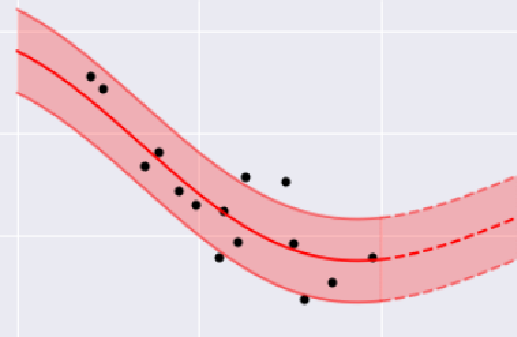
\includegraphics[scale=0.40]{motivation_fig1_1.pdf}}
\only<3>{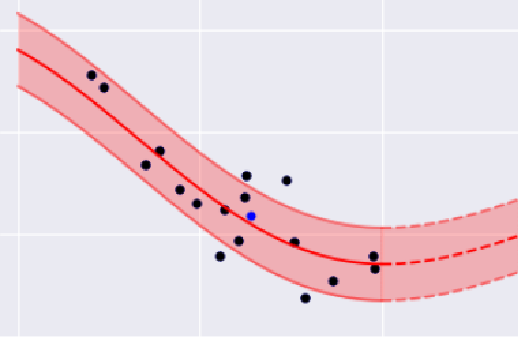
\includegraphics[scale=0.40, trim= 0mm 0mm 0mm 0mm, clip]{motivation_fig1_2.pdf}}
\only<4>{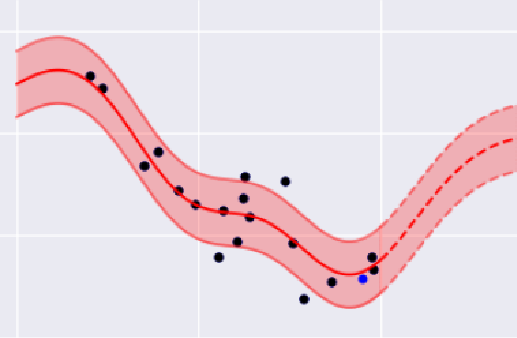
\includegraphics[scale=0.40, trim= 0mm 0mm 0mm 0mm, clip]{motivation_fig1_3.pdf}}
\only<5>{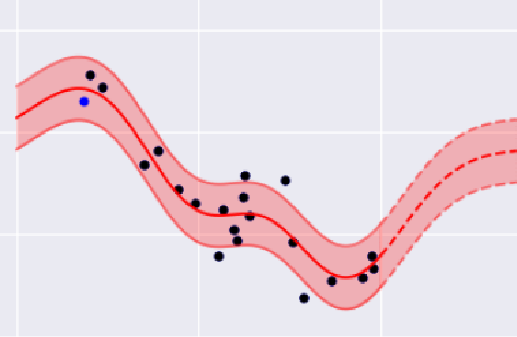
\includegraphics[scale=0.40, trim= 0mm 0mm 0mm 0mm, clip]{motivation_fig1_4.pdf}}
\only<6>{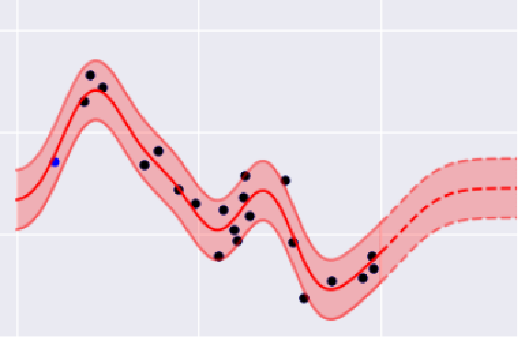
\includegraphics[scale=0.40, trim= 0mm 0mm 0mm 0mm, clip]{motivation_fig1_5.pdf}}
\visible<7->{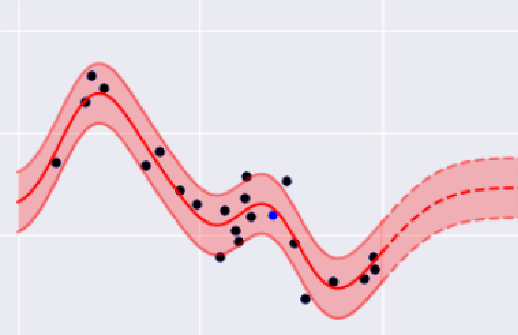
\includegraphics[scale=0.40, trim= 0mm 0mm 0mm 0mm, clip]{motivation_fig1_6.pdf}}

\end{itemize}

\item<8-> Many applications:

\begin{center}
\begin{tabular}{m{3cm} m{3cm} m{3cm}}
\visible<8->{Regression} & \visible<8->{Classification} & \\ 
%
\visible<8->{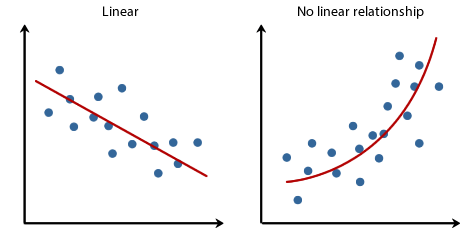
\includegraphics[scale=0.35,trim=90mm 0mm 0mm 8mm, clip]{motivation_fig2.png}} & \visible<8->{\includegraphics[scale=0.22,trim=120mm 0mm 230mm 12mm, clip]{motivation_fig3.pdf}} & \visible<8->{\pbox{5cm}{Density estimation\\[1mm]
Dimensionality reduction\\[1mm]
Solving differential equation\\[1mm]
...}}
\end{tabular}
\end{center}

\end{itemize}
\end{frame}
%----------------------------------------------------------------

%----------------------------------------------------------------
\begin{frame}
\setstretch{1.1}

\begin{itemize}\setlength\itemsep{2mm}
\item The key element of a GP is the {\color{navyblue} covariance function} as it encodes the covariance structure of function values.
%\item Covariance function is the main drawback of GPs in a direct implementation.

\item The covariance function generates the {\color{navyblue} covariance matrix} of the collection of function values.

\item Computing the posterior distribution of a GP {\color{navyblue} needs to invert the covariance matrix} $\to$\\ 
\begin{center}
{$\to$ \color{red} $O(n^3)$}
\end{center} 

\item This {\color{navyblue} limits their application} to rather small data sets (a few tens of thousands observations).

\item The problem {\color{navyblue} becomes more severe} with full Bayesian inference via sampling methods. 

\end{itemize}
\end{frame}
%----------------------------------------------------------------

%----------------------------------------------------------------
\begin{frame}
\setstretch{1.1}

\begin{itemize}\setlength\itemsep{3mm}
\item We focus on a low-rank representation of GPs using a {\color{navyblue} basis function approximation based on Hilbert space} {\color{darkgray} \citep{solin2018hilbert}}.

\item A basis function approximation to GPs has a linear functional structure:\\[2mm]
	\begin{itemize}\setlength\itemsep{1mm}
	\item Inference considerably faster.
	\item Improves sampling efficiency.
	\item Big benefit to be implemented in modular probabilistic programming frameworks. 
	\item Easier to be used as latent functions in non-Gaussian observational models. 
	\end{itemize}
\end{itemize}
\end{frame}
%----------------------------------------------------------------


\subsection*{Contribution}
%----------------------------------------------------------------
\begin{frame}
\frametitle{\normalsize Contribution}
\setstretch{1.1}

{\color{darkgray} \cite{solin2018hilbert} fully developed the mathematical theory behind this {\color{darkgray} low-rank GP}}. \\[4mm]

{\small \textit{\color{darkgray} Our contribution}:}\vspace{-2mm}
\begin{itemize}\setlength\itemsep{3mm}
\item A detailed analysis for its practical implementation in probabilistic programming.

\item The performance of the method depends on some interrelated key factors:\\[2mm]
	\begin{itemize}\setlength\itemsep{1mm}
	\normalsize
	\item {\color{navyblue} Discover the relationships} among these key factors in relation to accuracy and computational performance.
	\item {\color{navyblue} Practical recommendations} based on these relationships. %to improve performance and save computation time
	\item {\color{navyblue} Diagnosis} of the accuracy of the approximation.
	\end{itemize}

\item Implementation of the method in a fully probabilistic programming framework such as Stan.
\end{itemize}
\end{frame}
%----------------------------------------------------------------


\section{Gaussian process as a prior}

\subsection*{Gaussian process prior model}
%-----------------------------------------------------------------
\begin{frame}
\frametitle{\normalsize Gaussian process as a prior distribution for functions}
\setstretch{1.1}

\begin{itemize}\setlength\itemsep{2.5mm}
\item GP is a {\color{navyblue} stochastic process} which defines the distribution over a collection of random variables, $\left\lbrace  f(\bm{x}): \bm{x} \in \mathcal{X}\right\rbrace$ of a function $f:{\rm I\!R}^D \to {\rm I\!R}$ and some input domain $\mathcal{X} \subset {\rm I\!R}^D$.
%
\item Common notation:
%
\begin{align*}
f \sim \GP(m(\bm{x}), k(\bm{x}, \bm{x}'))
\end{align*}
%
\item The {\color{navyblue}mean} $m: {\rm I\!R}^D \to {\rm I\!R}$ and {\color{navyblue}covariance function}\, $k: {\rm I\!R}^D \times {\rm I\!R}^D \to {\rm I\!R}$ completely characterize the GP prior and control the a priori behavior of\, $f$.

\item Defining property: 
\vspace{-1mm}
%
\begin{align*}
\left\lbrace  f(\bm{x}_1), f(\bm{x}_2), \hdots, f(\bm{x}_N) \right\rbrace &\sim \Normal(\bm{\mu}, K),\\[1mm]
\mu_i &= m(\bm{x}_i),\\
\hspace{27mm} K_{i,j} &=\cov( f(\bm{x}_i),f(\bm{x}_j))=k(\bm{x}_i,\bm{x}_j).
\end{align*}
\end{itemize}
\end{frame}
%---------------------------------------------------------------

%---------------------------------------------------------------
\begin{frame}
\setstretch{1.1}

\begin{itemize}\setlength\itemsep{2mm}
\item Let \, $\bm{f}= \left\lbrace f(\bm{x}_1), f(\bm{x}_2), \hdots, f(\bm{x}_N) \right\rbrace$

\item Let \, $\bm{f}_1$ and \, $\bm{f}_2$ a partitioning of \, $\bm{f}= \bm{f}_1 \cup \bm{f}_2$:

\item<2-> Multivariate normal is {\color{navyblue} closed under conditioning}:
\end{itemize}

\vspace{-7mm}
\visible<2->{
\begin{align*}
\bm{f}_2 \mid \bm{f}_1 &\sim \Normal(\bm{\mu}, K),\\[1mm]
\bm{\mu} &= K_{2,1} K_{1,1}^{-1}(\bm{f}_1- \bm{\mu}_1) + \bm{\mu}_2,\\
K &= K_{2,2}-K_{2,1} K_{1,1}^{-1} K_{1,2}.
\end{align*}
}

\vspace{-10mm}
\begin{adjustwidth}{-1.6em}{-2em}
\begin{tabular}{ c c c }
\visible<3->{\scriptsize $\bm{f}\sim \Normal(\bm{\mu}, K)$} & \visible<4->{\scriptsize $\bm{f}_2 \mid \bm{f}_1$} & \visible<5->{\scriptsize $p(\bm{f}_2 \mid \bm{f}_1)$} \\
%
\visible<3->{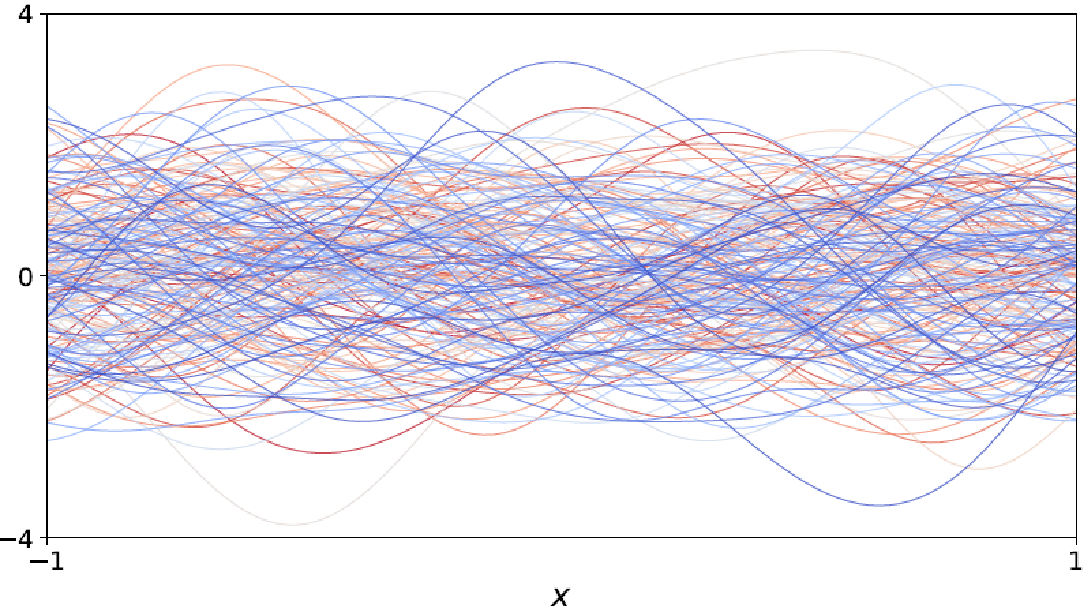
\includegraphics[width=4cm, trim = 7mm 12mm 1mm 0mm, clip]{GP_fig1.pdf}} & \visible<4->{\hspace{-3.5mm} 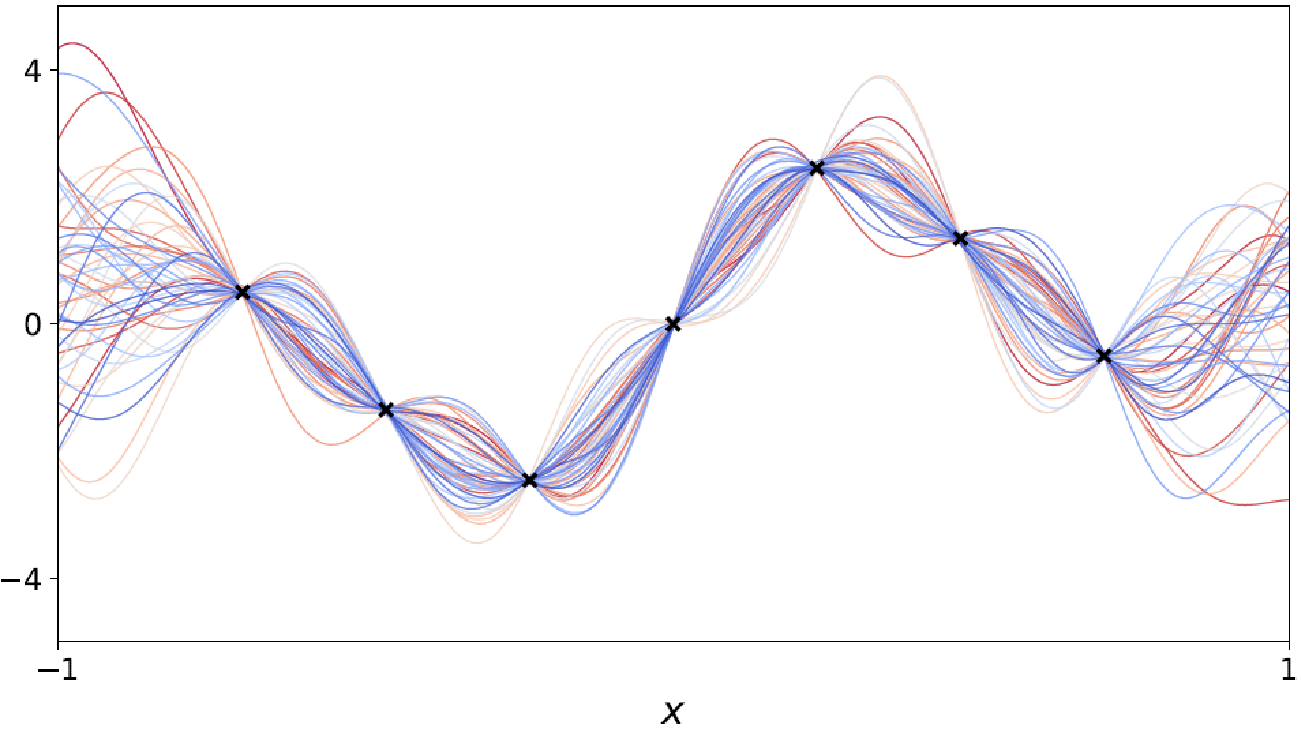
\includegraphics[width=4cm, trim = 8mm 13mm 1mm 0mm, clip]{GP_fig2.pdf}} & \visible<5->{\hspace{-3.5mm} 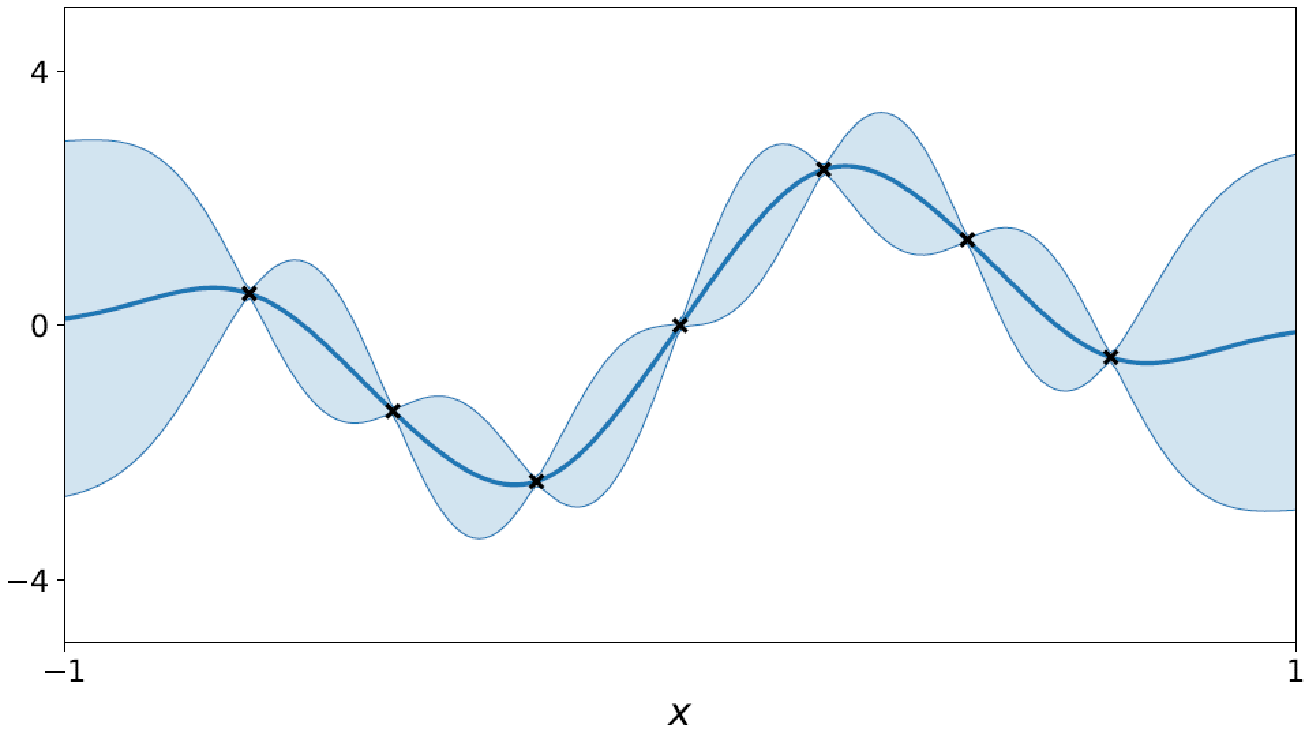
\includegraphics[width=4cm, trim = 9mm 13mm 2mm 0mm, clip]{GP_fig3.pdf}} \\[-2mm]
%
\visible<3->{\small $x$} & \visible<4->{\small $x$} & \visible<5->{\small $x$}
\end{tabular}
\end{adjustwidth}

\vspace{2mm}
\visible<5->{\scriptsize *These images belong to Nicolas Durrande, \textit{Course presentation in Gaussian Process Summer School 2019}, University of Sheffield.}
\end{frame}
%---------------------------------------------------------------

%---------------------------------------------------------------
\begin{frame}[t]\frametitle{\normalsize Latent Gaussian process model}
\setstretch{1.1}

\begin{itemize}\setlength\itemsep{2mm}
\item GP functions can be combined with noisy observations $\bm{y}$
\item and used as {\color{navyblue} latent functions} for observational models:
%
\vspace{2mm}
\begin{align*}
&{\Large p(y_i \mid f(\bm{x}_i),\phi)}\\[3mm]
&f:{\rm I\!R}^D \to {\rm I\!R}\; \text{is a latent function with a GP prior}
\end{align*}

\end{itemize}
\end{frame}
%---------------------------------------------------------------


\subsection*{Covariance function}
%---------------------------------------------------------------
\begin{frame}
\frametitle{\normalsize Covariance function}
\setstretch{1.1}

\vspace{-2mm}
\begin{adjustwidth}{-2.5em}{-0.5em}
\begin{itemize}\setlength\itemsep{2mm}
\item[] A covariance function\, $k : \mathcal{X} \times \mathcal{X} \to {\rm I\!R}$ maps a pair of inputs $x_1, x_2 \in \mathcal{X}$, from some input space $\mathcal{X} \in {\rm I\!R}^D$, to the real line ${\rm I\!R}$.\\[1mm]

	\begin{itemize}\setlength\itemsep{3mm}
	\item Encodes our {\color{navyblue} prior assumptions} about the variation of the function.
	
	\item Defines a {\color{navyblue} correlation structure} of function values.

	\item Generates the {\color{navyblue} covariance matrix} $K \in {\rm I\!R}^{N\times N}$, with\, $K_{ij}= \cov(f(\bm{x}_i),f(\bm{x}_j))= k(\bm{x}_i,\bm{x}_j)$.

	\item Covariance functions must be symmetric and Positive (Semi) Definite, such that,
	\begin{align*}
	\text{(Symmetric)}\hspace{5mm} &K = K^\intercal\\
	\text{(PSD)}\hspace{5mm} &\forall \bm{x} \neq 0 : \;\; \bm{x}^\intercal 		K \bm{x} \geq 0
	\end{align*}

	\item A covariance function is said to be {\color{navyblue} stationary} (invariant to translations) if \\[-1mm]% if it is only a function of difference of the input values,
	$$
	k(\bm{x},\bm{x}')= {\color{navyblue} k(\bm{x}-\bm{x}')}= k(\bm{\tau}), \;\; \bm{\tau} \in {\rm I\!R}^D
	$$

	\item A covariance functions is said to be {\color{navyblue} isotropic} (translation and rotation invariant) if\\[-1mm] % if it only depends on the input points through the norm of the difference, 
	$$
	k(\bm{x},\bm{x}') = {\color{navyblue} k(|\bm{x}-\bm{x}'|)} = k(r), \;\; r\in {\rm I\!R}
	$$ 
	
	\vspace{1mm}
	\hspace{20mm} \tiny$\bullet$ \scriptsize  {\color{navyblue} L2-norm $(|\bm{x}-\bm{x}'|_{L2})$}, although other types of distances can be considered.
	\end{itemize}
\end{itemize}
\end{adjustwidth}
\end{frame}
%---------------------------------------------------------------

%---------------------------------------------------------------
\begin{frame}
\setstretch{1.1}

The {\color{navyblue} Mat\'ern class} of isotropic covariance functions is given by:
 
\vspace{-5mm}
\begin{align*}
k_{\nu}(r)=\alpha \, \frac{2^{1-\nu}}{\Gamma(\nu)}\left(\frac{\sqrt{2\nu}r}{\ell}\right)^{\!\nu} \! K_{\nu} \left(\frac{\sqrt{2\nu}r}{\ell}\right)
\end{align*}

\vspace{-2mm}
\begin{itemize}\setlength\itemsep{1mm}
\item<1->$\nu > 0$\, is order of the kernel\; $\Rightarrow$\; {\color{navyblue} Samples paths are ($\nu-1$) times differentiable}\\[2mm]
\end{itemize}

\begin{adjustwidth}{-0.5cm}{-1cm}
\begin{tabular}{c c c c}
\small \visible<1->{$\nu=\infty$} & \small \visible<1->{$\nu=5/2$} & \small \visible<1->{$\nu=3/2$} & \small \visible<1->{$\nu=1/2$}\\[-1mm]
%
\scriptsize \visible<1->{Squared exponential} & \scriptsize \visible<1->{Matern52} & \scriptsize \visible<1->{Matern32} & \scriptsize \visible<1->{Matern12}\\[-1mm]
%
\visible<1->{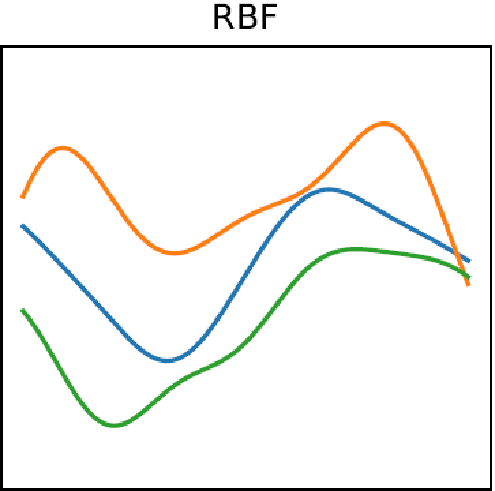
\includegraphics[width=2.8cm, trim = 0mm 0mm 0mm 5mm, clip]{covfun_fig1.pdf}} & \visible<1->{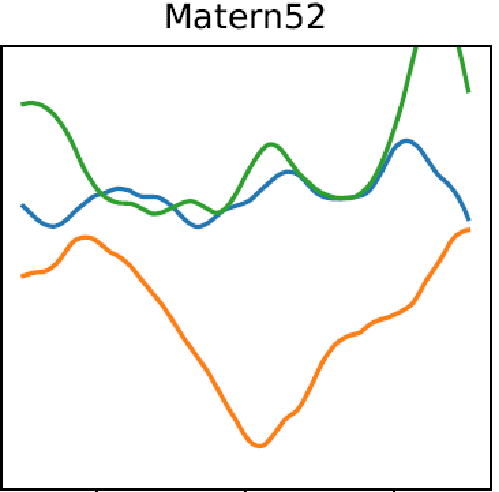
\includegraphics[width=2.8cm, trim = 0mm 0mm 0mm 5mm, clip]{covfun_fig2.pdf}} & \visible<1->{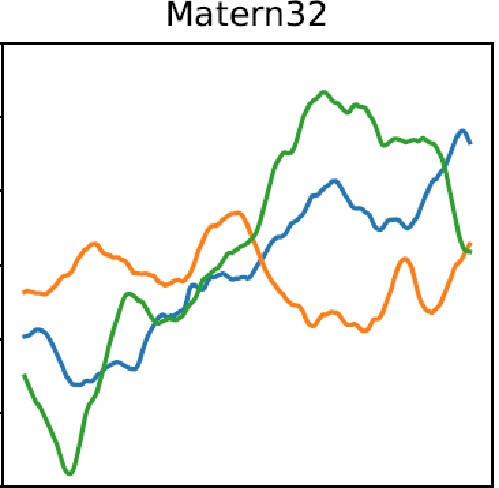
\includegraphics[width=2.8cm, trim = 0mm 0mm 0mm 5mm, clip]{covfun_fig3.pdf}} & \visible<1->{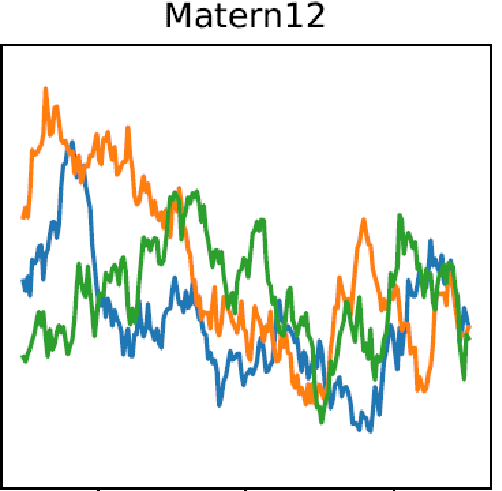
\includegraphics[width=2.8cm, trim = 0mm 0mm 0mm 5mm, clip]{covfun_fig4.pdf}}
\end{tabular}
\end{adjustwidth}

 {\scriptsize *These images belong to Nicolas Durrande, \textit{Course presentation in Gaussian Process Summer School 2019}, University of Sheffield.}
\end{frame}
%---------------------------------------------------------------

%---------------------------------------------------------------
\begin{frame}
\setstretch{1.1}

\begin{itemize}
\item $\ell > 0$,\: {\color{navyblue} length-scale} controls the {\color{navyblue} smoothness/wigglyness} of the function samples.\\[1mm]

\begin{itemize}\setlength\itemsep{0mm}
\item Using\, $\bm{\ell}=(\ell_1,\dots,\ell_D)\in {\rm I\!R}^D \rightarrow$  smoothness may vary across different input dimensions.
\end{itemize}

\vspace{1mm}
\begin{adjustwidth}{-3em}{-1em}

{ \color{black} \hspace{17mm} \centering $\ell=0.1$ \hspace{30mm} $\ell=0.3$ \hspace{30mm} $\ell=1.0$} \\[-4pt]
{\scriptsize \color{black} Squared exponential} \\
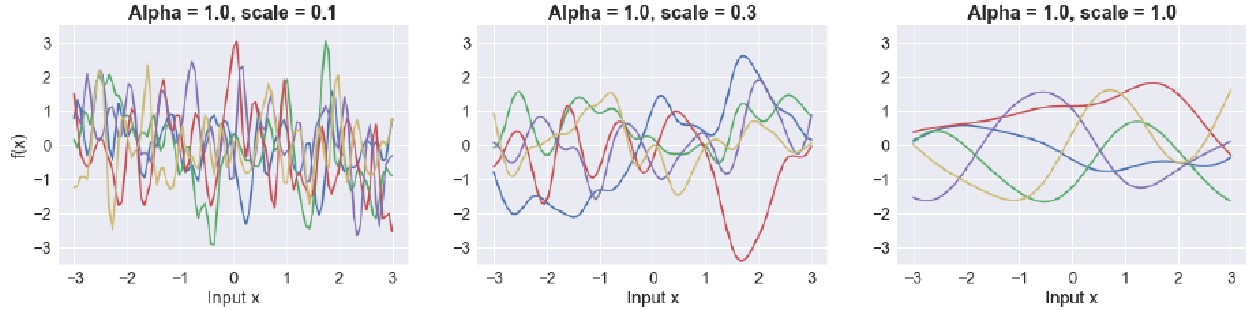
\includegraphics[width=12.5cm, trim = 0mm 3mm 0mm 5mm, clip]{covfun_fig5.pdf}

{\scriptsize \color{black} Mattern32}\\[1mm]
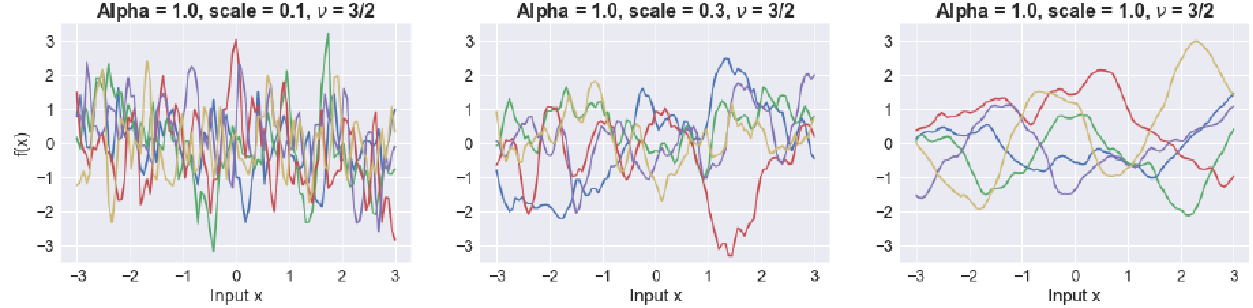
\includegraphics[width=12.5cm, trim = 0mm 0mm 0mm 5mm, clip]{covfun_fig6.pdf}

\end{adjustwidth}

\item $\alpha > 0$,\: {\color{navyblue} magnitude} or marginal variance of the process.
\end{itemize}
\end{frame}
%---------------------------------------------------------------


\subsection*{Computation requirements}
%---------------------------------------------------------------
\begin{frame}\frametitle{\normalsize Computation and learning hyperparameters}
\setstretch{1.1}

\begin{itemize}\setlength\itemsep{2mm}
\item Optimize kernel hyperparameters $\theta$ from data.

\item Ideally, specify priors $p(\theta)$ and compute the joint posterior:
 %
 \begin{align*}
	p(\bm{f},\theta \mid \bm{y}) = \frac{p(\bm{y}\mid \bm{f})\, p(\bm{f}\mid\theta) p(\theta)}{p(\bm{y})}
 \end{align*}
 
but marginal variance\, $p(\bm{y}) = \int p(\bm{y}\mid \bm{f})\, p(\bm{f}\mid\theta) p(\theta)\mathrm{d}\theta$\, is almost always intractable.

\vspace{5mm}
\item Using {\color{navyblue} Sampling methods} (MCMC), generates a sample from the unnormalized posterior, %as the posterior is proportional to the likelihood and priors:
%
\begin{align*}
p(\bm{f},\theta\mid y) \propto p(y\mid\bm{f})p(\bm{f}\mid\theta)p(\theta)
\end{align*}

\begin{itemize}\setlength\itemsep{2mm}
\item Evaluating\, $p(\bm{f} \mid\theta) \sim \Normal(\bm{\mu}, K(\theta))$\,  in every sampling step is a\, {\color{navyblue} $O(N^3)$ operation}.\\[2mm]

\vspace{-1mm}
\item MCMC {\color{navyblue} is not the fastest} approach, but allows {\color{navyblue} accurate inference}.
\item It is commonly referred as {\color{navyblue}full Bayesian inference}.
\end{itemize}
\end{itemize}
\end{frame}
%---------------------------------------------------------------

%---------------------------------------------------------------
\begin{frame}
\setstretch{1.1}

\begin{itemize}\setlength\itemsep{2mm}
\item {\color{navyblue} Maximum a posteriori} (MAP) optimizes the posterior distribution over the parameter space.
 %
 \begin{gather*}
	p(\theta \mid \bm{y}) = \frac{\int p(\bm{y}\mid \bm{f})\, p(\bm{f}\mid \theta)\, p(\theta) \operatorname{d}\bm{f}}{p(\bm{y})}  = \frac{p(\bm{y}\mid \theta)\, p(\theta)}{p(\bm{y})} \propto p(\bm{y}\mid \theta)\, p(\theta)\\[3mm]
%
 \hat{\theta} = \argmax_\theta \left( \ln \left( p(\bm{y}\mid \theta)\, p(\theta)\right) \right) = \argmax_\theta \left( \ln p(\bm{y}\mid \theta) + \ln p(\theta) \right)
 \end{gather*}

\item {\color{navyblue} Maximum likelihood} (ML) methods optimize the likelihood function over the parameter space.\\[1mm]
 ML $\Leftrightarrow$ MAP with $p(\theta)\propto 1$.
 %
 \begin{gather*}
 \hat{\theta} = \argmax_\theta \left( \ln p(\bm{y}\mid \theta) \right)
 \end{gather*}

\item e.g. with Gaussian observational model, to optimize $p(\bm{y}\mid \theta)$ wrt. $\theta$ using gradient based methods,
%
\begin{align*}
\nabla_\theta \ln p(\bm{y}\mid \theta)= \nabla_\theta\; -\frac{N}{2}\ln(2\pi)-\frac{1}	{2}\ln|\sigma^2I+K|-\frac{1}{2}\bm{y}^\intercal(\sigma^2I+K)^{-1}\bm{y},
\end{align*}
%
the {\color{navyblue} covariance matrix needs to be inverted} which is an $O(N^3)$ operation.

\end{itemize}
\end{frame}
%---------------------------------------------------------------

%---------------------------------------------------------------
\begin{frame}
\setstretch{1.1}

{\color{navyblue} MCMC}, {\color{navyblue} MAP} and {\color{navyblue} ML} need to invert the covariance matrix with cost $O(N^3)$.\\[0.7cm]

$O(N^3)$:
	\begin{itemize}\setlength\itemsep{2mm}
	\item[] $N < 1000 \to$ Fine
	\item[] $N < 10000 \to$ Slow, but possible
	\item[] $N > 10000 \to$ Prohibitively slow
	\end{itemize}
\end{frame}
%---------------------------------------------------------------

%---------------------------------------------------------------
\begin{frame}
\setstretch{1.1}

\textsc{\small Other approximate methods for Bayesian inference:}
\begin{itemize}\setlength\itemsep{2mm}
\item {\color{navyblue} Laplace approximation}
\item {\color{navyblue} Expectation propagation}
\item {\color{navyblue} Variational Bayes}
\end{itemize}
\end{frame}
%---------------------------------------------------------------


\subsection*{Related low-rank GP methods}
%---------------------------------------------------------------
\begin{frame}\frametitle{\normalsize Related low-rank approximate GP methods}
\setstretch{1.1}

\begin{itemize}\setlength\itemsep{2mm}
\item {\color{navyblue} Sparse GPs} are based on low-rank approximations of the covariance matrix with $m \ll n$ inducing points, and computational complexity of $O(nm^2 + m^3)$ \\[1mm]
	%
	\begin{itemize}\setlength\itemsep{2mm}
		\item Inducing points-based sparse approximation
		\item Structured kernel interpolation method
	\end{itemize}

\item {\color{navyblue} Basis function approximations} with $m \ll n$ basis functions and computational complexity of $O(nm+m)$.\\[1mm]
	%
	\begin{itemize}\setlength\itemsep{2mm}
	\item Spectral analysis and series expansions of GPs
	\item Sparse spectrum GPs
	\item Variational Fourier feature approximation for GPs
	\end{itemize}
	
\item ...

\end{itemize}

\centering
\begin{tcolorbox}[boxrule=0.5pt,colframe=blue!20, colback=blue!5]
A Hilbert space method to approximate GPs is a {\color{navyblue} basis function approximation via Laplace eigenfunctions} for stationary covariance functions.
\end{tcolorbox}
\end{frame}
%---------------------------------------------------------------


\subsection*{Spectral density function}
%---------------------------------------------------------------
\begin{frame}\frametitle{\normalsize Spectral density function}
\setstretch{1.1}

\vspace{-2mm}
Stationary covariance functions can be represented in terms of their {\color{navyblue} spectral density functions}.

\vspace{2mm}
\begin{thm}[Bochner]
Any {\color{navyblue} stationary covariance function}\, $k:{\rm I\!R}^{D} \to {\rm I\!R}$\, and its {\color{navyblue} spectral density}\, $S:{\rm I\!R}^{D} \to {\rm I\!R}$\, are Fourier duals.
\vspace{-1mm}
\begin{align*}
k(\bm{\tau})=& \int S(\bm{\omega}) e^{2\pi i \bm{\omega} \cdot \bm{\tau}} d\bm{\omega}, \hspace{10mm} \text{(Inverse Fourier Transform)} \nonumber \\
%
S(\bm{\omega})=& \int k(\bm{\tau}) e^{-2\pi i \bm{\omega} \cdot \bm{\tau}} d\bm{\tau}. \hspace{10mm} \text{(Fourier Transform)}  \nonumber
\end{align*}

where\, $\bm{\tau}=\bm{x}-\bm{x}' \in {\rm I\!R}^{D}$, and\, $\bm{\omega} \in {\rm I\!R}^{D}$\, is a frequency.
\end{thm}

\vspace{2mm}
\begin{adjustwidth}{-0.2em}{-0.2em}
\begin{itemize}\setlength\itemsep{2mm}
\item Given a {\color{navyblue} kernel} $k(\bm{\tau})$, the {\color{navyblue} frequencies} that it considers can be obtained by solving the FT.

\item Given a {\color{navyblue} spectral density} $S(\bm{\omega})$, its {\color{navyblue} similarity function} can be obtained by solving the IFT.

\item We can custom spectral densities (frequencies) and get new kernels ({\color{navyblue} kernel learning}).
\end{itemize}
\end{adjustwidth}

\end{frame}
%---------------------------------------------------------------


\section[Hilbert space approximate GP model (HSGP)]{Hilbert space approximate Gaussian process model (HSGP)}

\subsection*{HSGP model}
%---------------------------------------------------------------
\begin{frame}\frametitle{\normalsize Hilbert space approximate GP model (HSGP)}
\setstretch{1.1}

\begin{itemize}\setlength\itemsep{2mm}

\item The covariance function is represented as a {\color{navyblue} infinite series expansion} of eigenfunctions $\phi_j(x)$ scaled by the spectral density\, $S_{\theta}(\sqrt{\lambda_j})$ {\color{darkgray} \citep{solin2018hilbert}}:
%
\begin{align*}
k(x,x') = \sum_{j=1}^\infty S_{\theta}(\sqrt{\lambda_j}) \phi_j(x) \phi_j(x'), \hspace{10mm} x,x' \in [-L,L]
\end{align*} 

\item We choose the {\color{navyblue} eigenvalues} $\lambda_j$ and {\color{navyblue} eigenfunctions} $\phi_j(x)$ of the Laplacian operator $-\nabla^2$:
%
\begin{align*}
-\nabla^2 \phi_j(x)&=\lambda_j \phi_j(x), \hspace{0.8cm}  x \in [-L,L] \\ 
\hspace{6mm}\phi_j(x)&=0, \hspace{1.6cm} x \notin [-L,L]
\end{align*}

given by:\\[-5mm]
%
\begin{gather*}
\lambda_j=\left(\frac{j\pi}{2L}\right)^2 \hspace{10mm}
\phi_j(x)=\sqrt{\frac{1}{L}} \text{sin}\left(\sqrt{\lambda_j}(x+L)\right)
\end{gather*}

\item $L > 0$ represents the {\color{navyblue} boundaries} where this representation is valid.
\end{itemize}
\end{frame}
%---------------------------------------------------------------

%---------------------------------------------------------------
\begin{frame}[t]
\setstretch{1.1}

\vspace{-1mm}
\begin{itemize}\setlength\itemsep{1mm}
\item<1-> To make this representation useful we can truncated the sum to the first $m$ terms:
%
\vspace{-1mm}
\begin{align*}
k(x,x') \approx \sum_{j=1}^m S_{\theta}(\sqrt{\lambda_j}) \phi_j(x) \phi_j(x'), \hspace{10mm} x,x' \in [-L,L]
\end{align*}
\end{itemize}

\vspace{-10mm}
\begin{adjustwidth}{-2em}{-1em}
\begin{tabular}{c c}
 \only<2-6>{$\phi_j(x)$} & \visible<5->{$S_{\theta}(\sqrt{\lambda_j})$} \\
 %
 \only<2>{\hspace{2mm}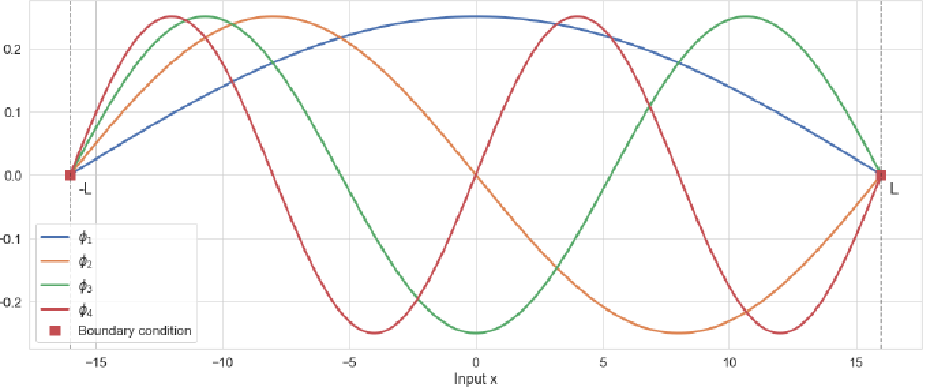
\includegraphics[width=6cm, trim = 0mm 0mm 0mm 0mm, clip]{HSGP_fig1_1.pdf}}
\only<3>{\hspace{1mm}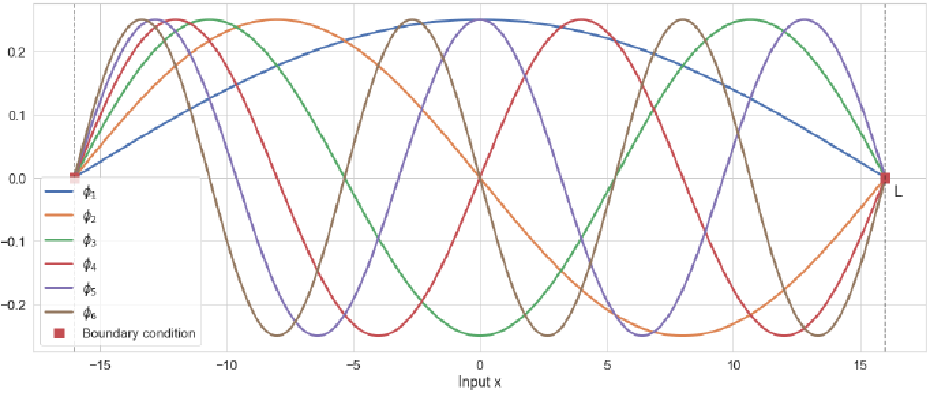
\includegraphics[width=6cm, trim = 0mm 0mm 0mm 0mm, clip]{HSGP_fig1_2.pdf}}
\only<4-6>{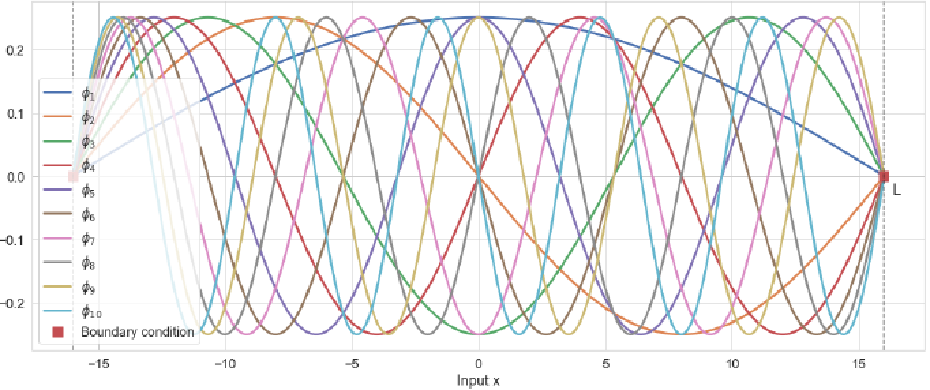
\includegraphics[width=6cm, trim = 0mm 0mm 0mm 0mm, clip]{HSGP_fig1_3.pdf}} & \visible<5->{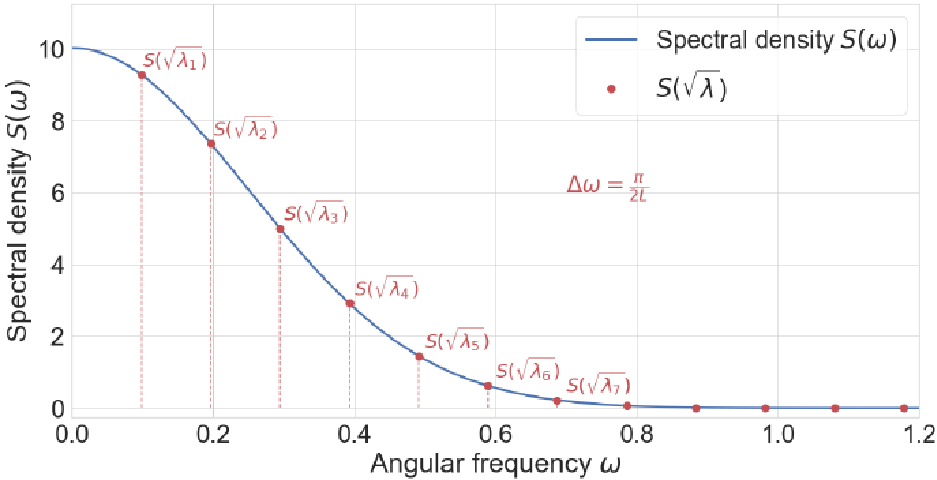
\includegraphics[width=6.1cm, trim = 0mm 0mm 0mm 0mm, clip]{HSGP_fig2.pdf}}\\[-2mm]
\end{tabular}
\end{adjustwidth}

\begin{itemize}\setlength\itemsep{1mm}
\item<6-> $S_{\theta}(\sqrt{\lambda_j})$ decays rapidly to zero.
\item<6-> This rate of dacay depends on the lenghtscale of $k$ or smoothness of the function to be learned.
\item<6-> A finite number $m$ of terms for an accurate approximation.
\item<6-> As long as $x_i$ are not too close to the boundaries $-L$ and $L$ of $\Omega$.
\end{itemize}
\end{frame}
%---------------------------------------------------------------

%---------------------------------------------------------------
\begin{frame}[t]
\setstretch{1.1}

\begin{itemize}\setlength\itemsep{2mm}

\item This representation\, $k(x,x') \approx \sum_{j=1}^m S_{\theta}(\sqrt{\lambda_j}) \phi_j(x) \phi_j(x')$\, leads to the\\ {\color{navyblue} linear representation} of the function\, $f$:
%
\begin{align*}
f(x) \approx \sum_{j}^m \phi_j(x) \beta_j, \hspace{10mm} \beta_j \sim \Normal(0,S_{\theta}(\sqrt{\lambda_j})).
\end{align*}
\end{itemize}

%\vspace{10mm}
%\begin{itemize}\setlength\itemsep{1mm}
%\small
%\item Several common GP approximations lead to approximations of similar form (i.e. sparse GPs etc).
%\item All of them require a Cholesky factorization or eigendecomposition of the kernel matrix.
%\item However, Hilbert space methods give analytical expressions for both eigenfunctions and variance of the weights $\beta_j$.
%\end{itemize}


\begin{tcolorbox}[colframe=blue!20, colback=white, title=\small Properties of the method, colbacktitle=lightblue, coltitle=black, boxrule=0.5pt]
\setstretch{1.1}
\begin{itemize}\setlength\itemsep{1.5mm}
\item[+] The basis functions $\phi_j(x)$ do not depend on the hyperparameters, so they just need to be computed once with cost $O(nm)$.

\item[+]  All dependencies on the hyperparameters is through the variance of the weights $\beta_j$.

%\item[+]  In every step of the sampler the computational complexity is that of a linear model $O(nm)$.

%\item[+] $f(x)$ is naturally in the {\color{navyblue} non-centered parameterization form} with independent prior distribution on $\beta_j$ which makes posterior inference easier. %\citep[see, e.g., ][]{Betancourt+Girolami:2019} 

\item[+]  The parameter posterior\, $p(\bm{\beta}|\bm{y})$ is\, $m$-dimensional ($m\ll n$), which makes posterior inference easier.

\item[+] Trade-off between accuracy and computation.

\item[-] Scales badly with the number of input dimensions $D$.

\item[-] In practice,\, $D>3$\, starts to be too computationally demanding, even for smooth functions.
\end{itemize}
\end{tcolorbox}
\end{frame}
%---------------------------------------------------------------


\subsection*{Aim of the study}
%---------------------------------------------------------------
\begin{frame}
\setstretch{1.1}

\begin{tcolorbox}[colframe=blue!20, colback=white, title=\small Aim of the study, colbacktitle=lightblue, coltitle=black, boxrule=0.5pt]
\setstretch{1.1}

Determine the minimum $m$ ({\color{navyblue} basis functions}) and valid $L$ ({\color{navyblue} boundary}) to obtain accurate approximations, as a function of the {\color{navyblue} lengthscale}.

\begin{enumerate}
\item How many basis functions $m$ are needed for a good approximation?

\item Which is the effect of the boundary box $L$ on the approximation?

\item Which are valid values for the boundary box $L$?

\item How $m$ and $L$ relate to each other and to the wigglyness of the function to be learned?
\end{enumerate}
\end{tcolorbox}
\end{frame}
%---------------------------------------------------------------


\subsection*{Generalization to multidimensional input space}
%---------------------------------------------------------------
\begin{frame}\frametitle{\normalsize Generalization to multidimensional input space}
\setstretch{1.1}

\begin{itemize}\setlength\itemsep{2mm}
\item Regular and compact domain\, $\Omega=[-L_1,L_1] \times \dots \times [-L_D,L_D] \subset {\rm I\!R}^D$

\item The total number of eigenfunctions and eigenvalues is\, $m^{\ast} = \prod_{d=1}^{D} m_d$ %that is possible combinations of univariate eigenfunctions over all dimensions

\vspace{4mm}
\begin{columns}
\column{0.3\textwidth}
\centering
 {\small e.g. $D=2$:} \\[1mm]
 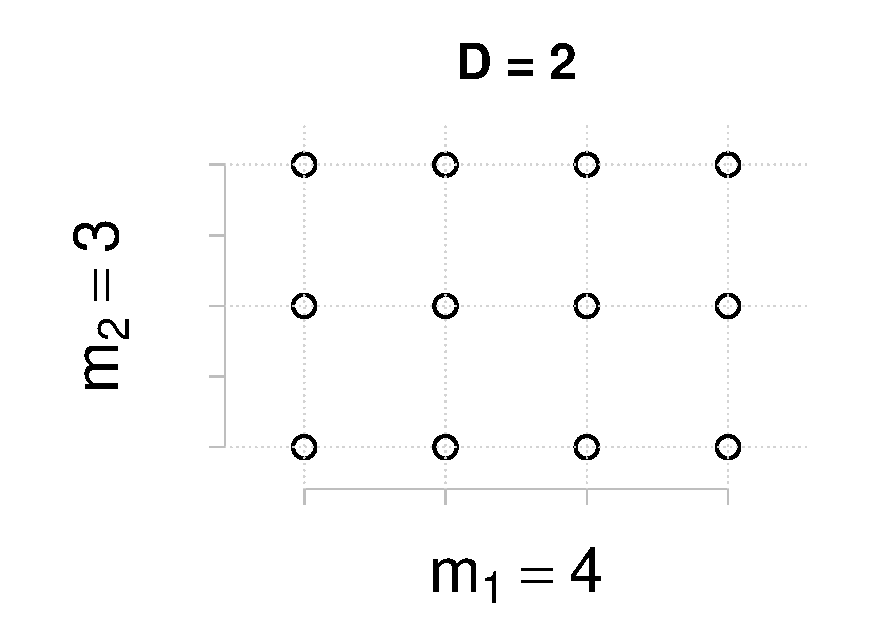
\includegraphics[width=4cm, trim = 0mm 0mm 0mm 20mm, clip]{HSGP_fig3.pdf}

\column{0.5\textwidth}
\begin{align*}\small
\mathbb{S}^\intercal=
\left[ {\begin{array}{cccccccccccc}
1 & 1 & 1 & 2 & 2 & 2 & 3 & 3 & 3 & 4 & 4 & 4  \\
1 & 2 & 3 & 1 & 2 & 3 & 1 & 2 & 3 & 1 & 2 & 3  
\end{array} } \right] \in {\rm I\!R}^{2\times 12}
\end{align*} 
\end{columns}

\vspace{-2mm}
\item Thus, for\, $\bm{x}=\{x_d\}_{d=1}^D \in \Omega$\, and\, $j=1,\ldots,m^{\ast}$, we have:
%
\begin{align*}
\bm{\lambda}^{\ast}_j &= \left\{ \lambda_{\mathbb{S}_{jd}} \right\}_{d=1}^D =  \left\{ \left(\tfrac{\pi \mathbb{S}_{jd}}{2L_d}\right)^2 \right\}_{d=1}^D \\[1mm]
%
\phi^{\ast}_j(\bm{x}) &= \prod_{d=1}^{D} \phi_{\mathbb{S}_{jd}}(x_d) = \prod_{d=1}^{D} \sqrt{\frac{1}{L_d}} \text{sin}\left(\sqrt{\lambda_{\mathbb{S}_{jd}}}(x_d+L_d)\right)
\end{align*}

\end{itemize}
\end{frame}
%---------------------------------------------------------------

%---------------------------------------------------------------
\begin{frame}
\setstretch{1.1}

\begin{itemize}\setlength\itemsep{4mm}
\item And the approximate covariance function\, $k(\bm{x},\bm{x}',\theta)$\, and\, $f(\bm{x})$:
%
\begin{align*}
k(\bm{x},\bm{x}') &\approx \sum_{j=1}^{m^{\ast}} 
S^{\ast}_{\theta}\left(\sqrt{\bm{\lambda}^{\ast}_j}\right)
\phi^{\ast}_j(\bm{x}) \phi^{\ast}_j(\bm{x}') \\
%
f(\bm{x}) &\approx \sum_{j=1}^{m^{\ast}} 
\left( S^{\ast}_{\theta} \left(\sqrt{\bm{\lambda}^{\ast}_j} \right)\right)^{1/2}
\phi^{\ast}_j(\bm{x}) \beta_j
\end{align*}

where $S^{\ast}_{\theta}$ is the spectral density of the $D$-dimensional covariance function.

\vspace{2mm}
\item The number of multivariate basis functions,\, $m^{\ast} = \prod_{d=1}^{D} m_d$,\, {\color{navyblue} grows exponentially} with respect to $D$.\\[-2mm]
 \[O(nm^*+m^*)\]

\item In practice,\, $D>3$\, starts to be too computationally demanding, even for smooth functions.

\end{itemize}
\end{frame}
%---------------------------------------------------------------


\section{Performance analysis of HSGP}
%---------------------------------------------------------------
\begin{frame}\frametitle{\normalsize Performance analysis of HSGP}
\setstretch{1.1}

The {\color{navyblue} performance}, {\color{navyblue} accuracy} and {\color{navyblue} speed} of the method mainly depends on:
%
\begin{center}
\begin{tabular}{ l l l}
 \pbox{5cm}{Number of basis functions ($m$) \\ Boundary box ($L$)} & $\Leftrightarrow$ & Smoothness ($\ell$)
\end{tabular}
\end{center}

\begin{tcolorbox}[colframe=blue!20, colback=white, title=Objectives, colbacktitle=lightblue, coltitle=black, boxrule=0.5pt]
\setstretch{1.1}
\begin{enumerate}\setlength\itemsep{2mm}
\item Analysis of the effects of\, $m$\, and\, $L$ on the approximation.
\item A model gathering the relationships among\, $m$, $L$\, and\, $\ell$ in terms of an accurate approximation \\

 \centering $\Downarrow$
 \\[2mm]
 \begin{center}
 \begin{tabular}{@{}l@{}}
 \tabitem make useful and valuable {\color{navyblue} recomendations} \\
 \tabitem make {\color{navyblue} diagnosis} of the performance \\
 \tabitem save time of computation 
 \end{tabular}
 \end{center}
 
\end{enumerate}
\end{tcolorbox}
\end{frame}
%---------------------------------------------------------------


\subsection*{Effects of $m$ and $L$}
%---------------------------------------------------------------
\begin{frame}
\setstretch{1.1}

\begin{enumerate}
\item<1-> \textbf{Effects of}\, $m$\, \textbf{and}\, $L$\, \textbf{on the approximation}

\vspace{3mm}
 \pbox{6cm}{Boundary box\, $\Omega \in [-L,L]$ \\ Desired input domain\, $\Phi \in [-S,S]$}\;\;  $\to$\;\;  $L=c \cdot S$, \hspace{3mm} $c \geqslant 1$, \hspace{1mm} $c \equiv$ {\color{navyblue} Boundary factor}

\vspace{3mm}
\begin{itemize}\setlength\itemsep{1mm}
\item<2-> \normalsize Effect of\, $m$\; ($c$ is fixed)

\begin{adjustwidth}{-4.7em}{-3em}
\centering
{\scriptsize \hspace{5mm} Covariance \hspace{30mm} \visible<3->{Mean function} \hspace{27mm} \visible<4->{Standard deviation}}\\[-4mm]
%
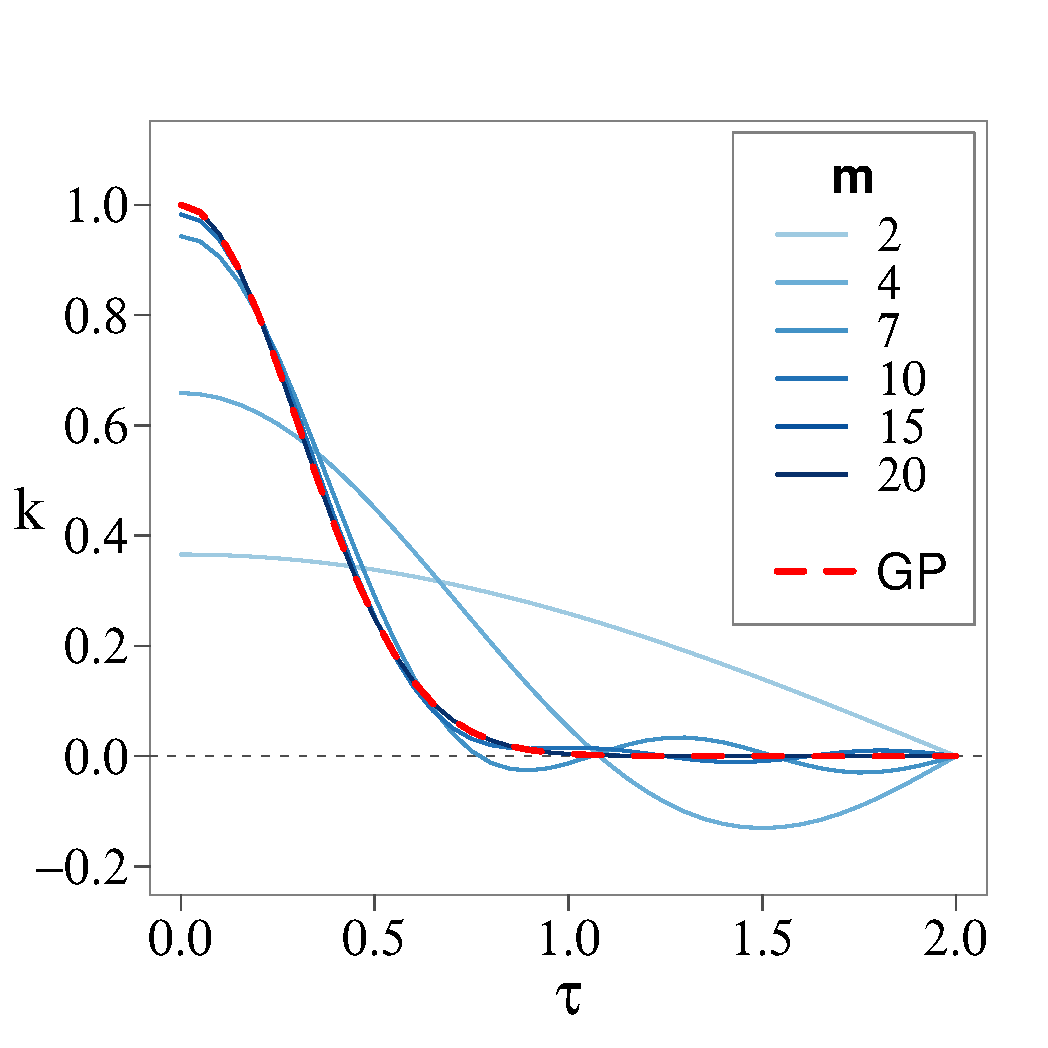
\includegraphics[scale=0.23, trim = 0mm 0mm 0mm 0mm, clip]{ch5_fig1_Cov_J.pdf}
\visible<3->{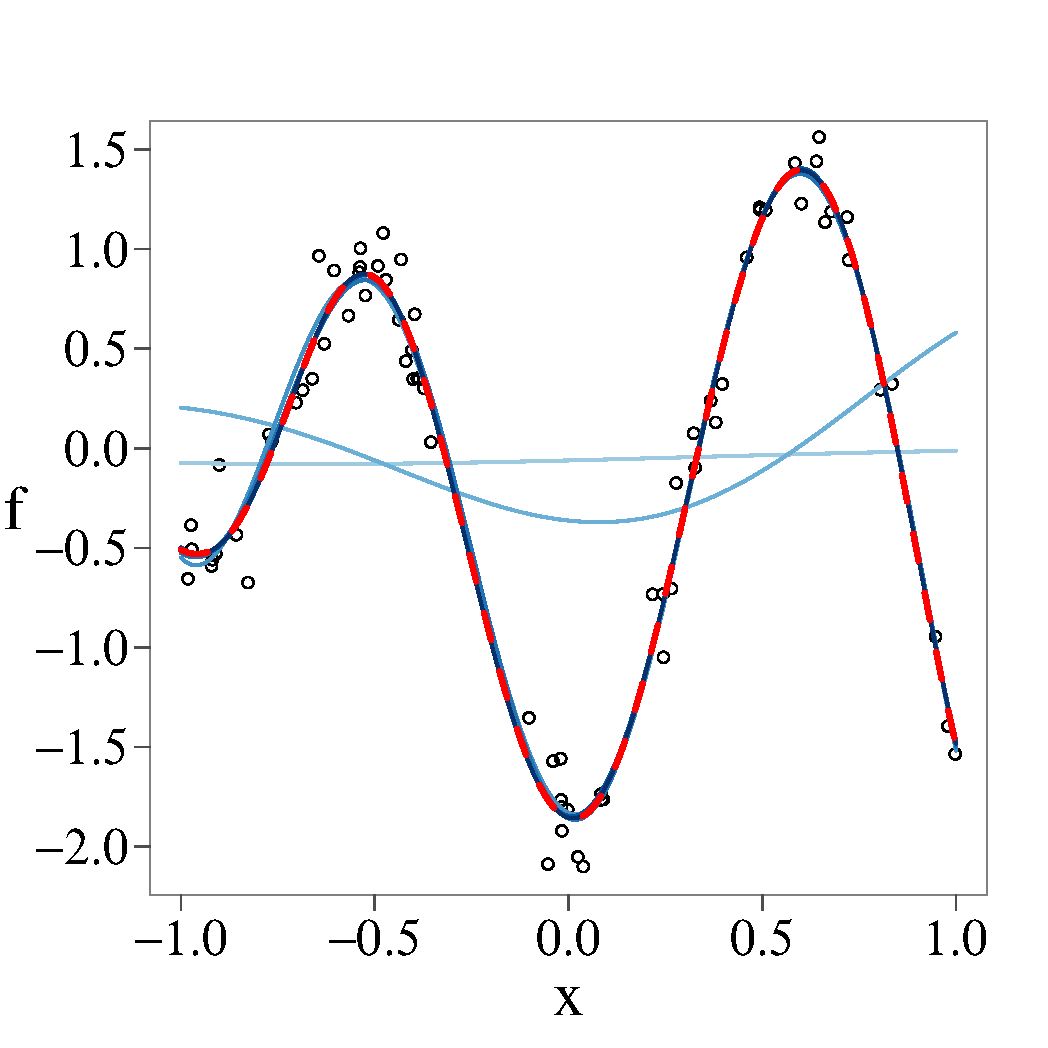
\includegraphics[scale=0.23, trim = 0mm 0mm 0mm 0mm, clip]{ch5_fig1_Post_J.pdf}}
\visible<4->{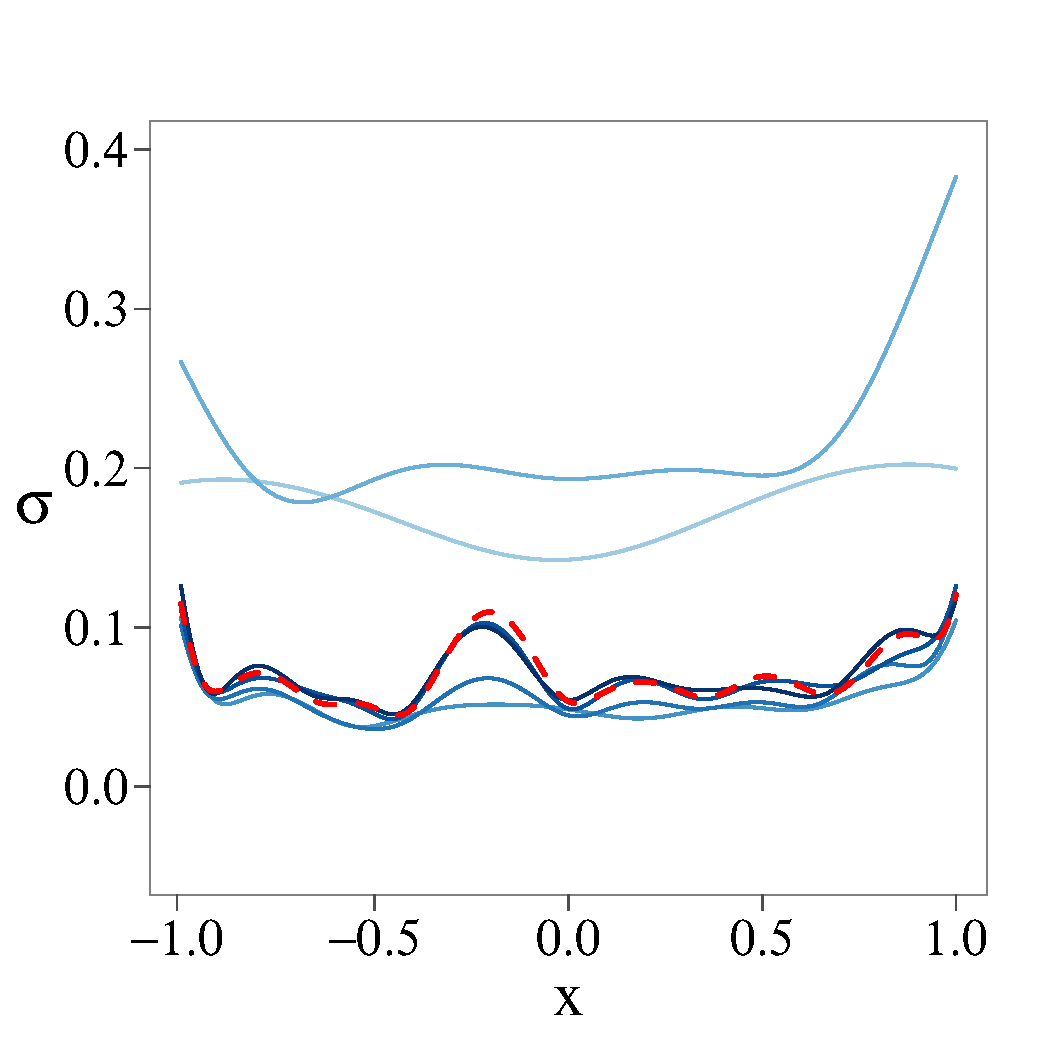
\includegraphics[scale=0.23, trim = 0mm 0mm 0mm 0mm, clip]{ch5_fig1_Sigma_J.pdf}}
\end{adjustwidth}

\normalsize 
\item<3-> $m$\, affects the smoothness of the posterior function:\; The lower\, $m$,\, the smoother the posterior.
\item<3-> The higher the wigglyness of the function to be learned, the higher\, $m$\, is required.
\item<4-> $m$\, affects the uncertainty as well (obviously).
\item<4-> The approximation is more sensitive in the uncertainty than in mean.
\end{itemize}
\end{enumerate}
\end{frame}
%---------------------------------------------------------------

%---------------------------------------------------------------
\begin{frame}
\setstretch{1.1}

\begin{itemize}\setlength\itemsep{2mm}
\item \normalsize Effect of\, $c$\; ($m$ is fixed)\\[2mm]

\begin{adjustwidth}{-2.7em}{-3em}
\begin{center}
{\scriptsize \hspace{5mm} Covariance \hspace{30mm} \visible<1->{Mean function} \hspace{27mm} \visible<2->{Standard deviation}}\\[-4mm]
%
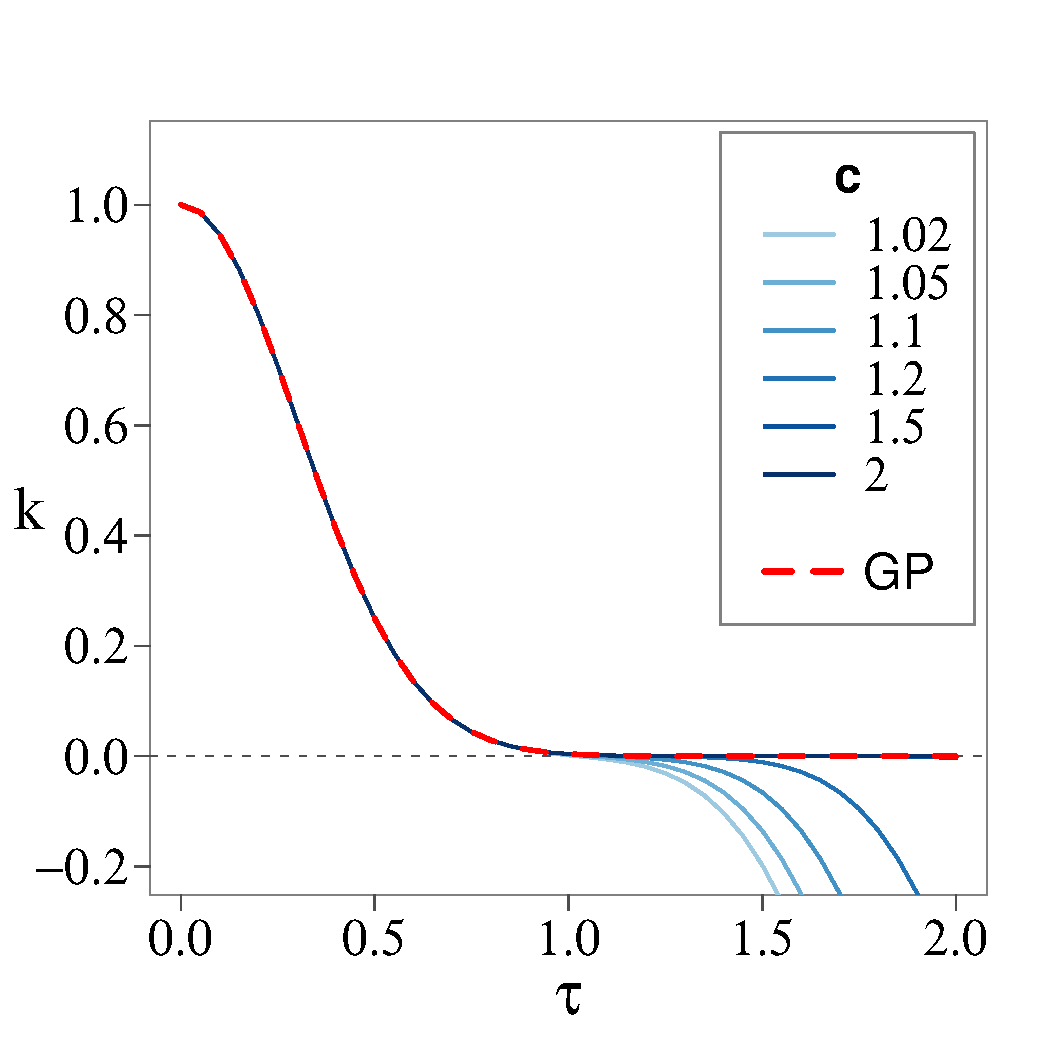
\includegraphics[scale=0.23, trim = 0mm 0mm 0mm 0mm, clip]{ch5_fig2_Cov_L.pdf}
\visible<1->{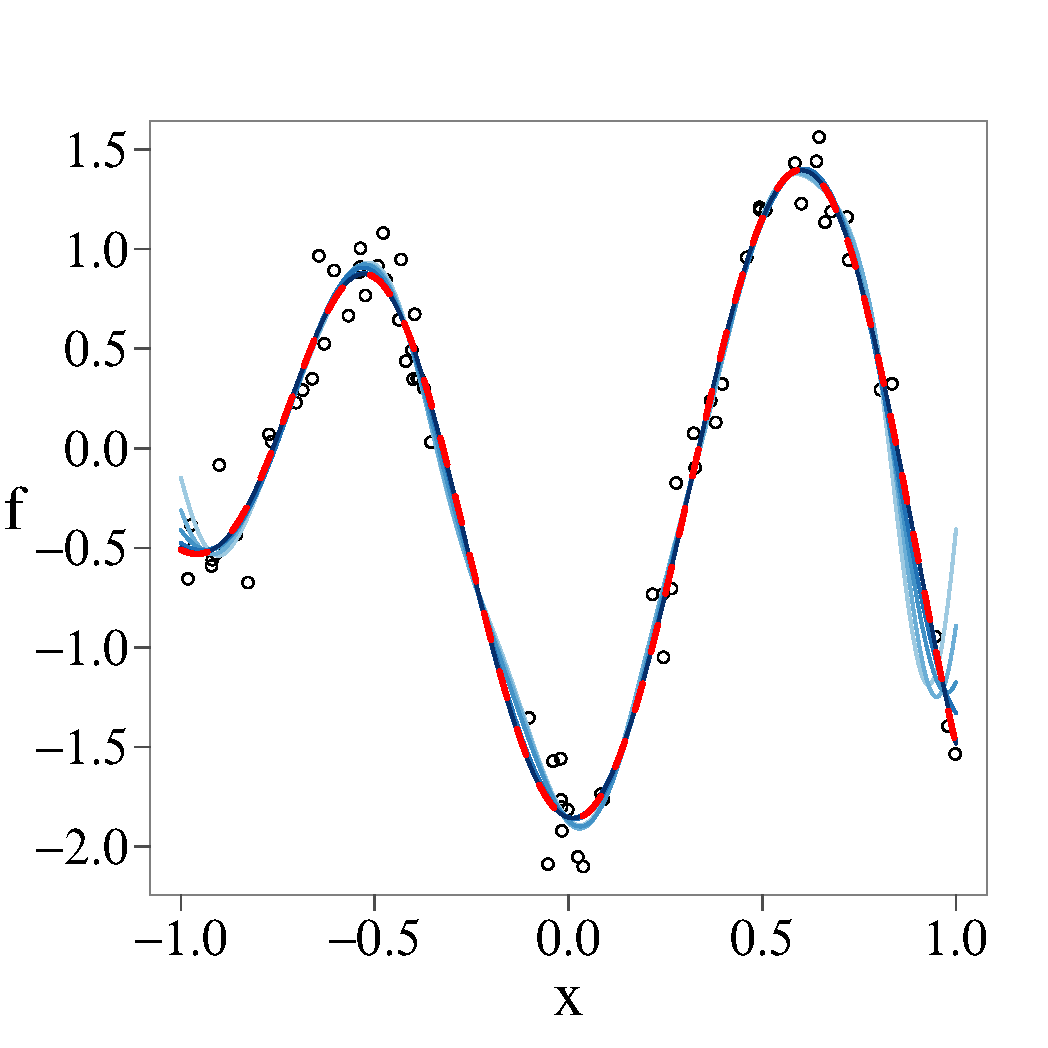
\includegraphics[scale=0.23, trim = 0mm 0mm 0mm 0mm, clip]{ch5_fig2_Post_L.pdf}}
\visible<2->{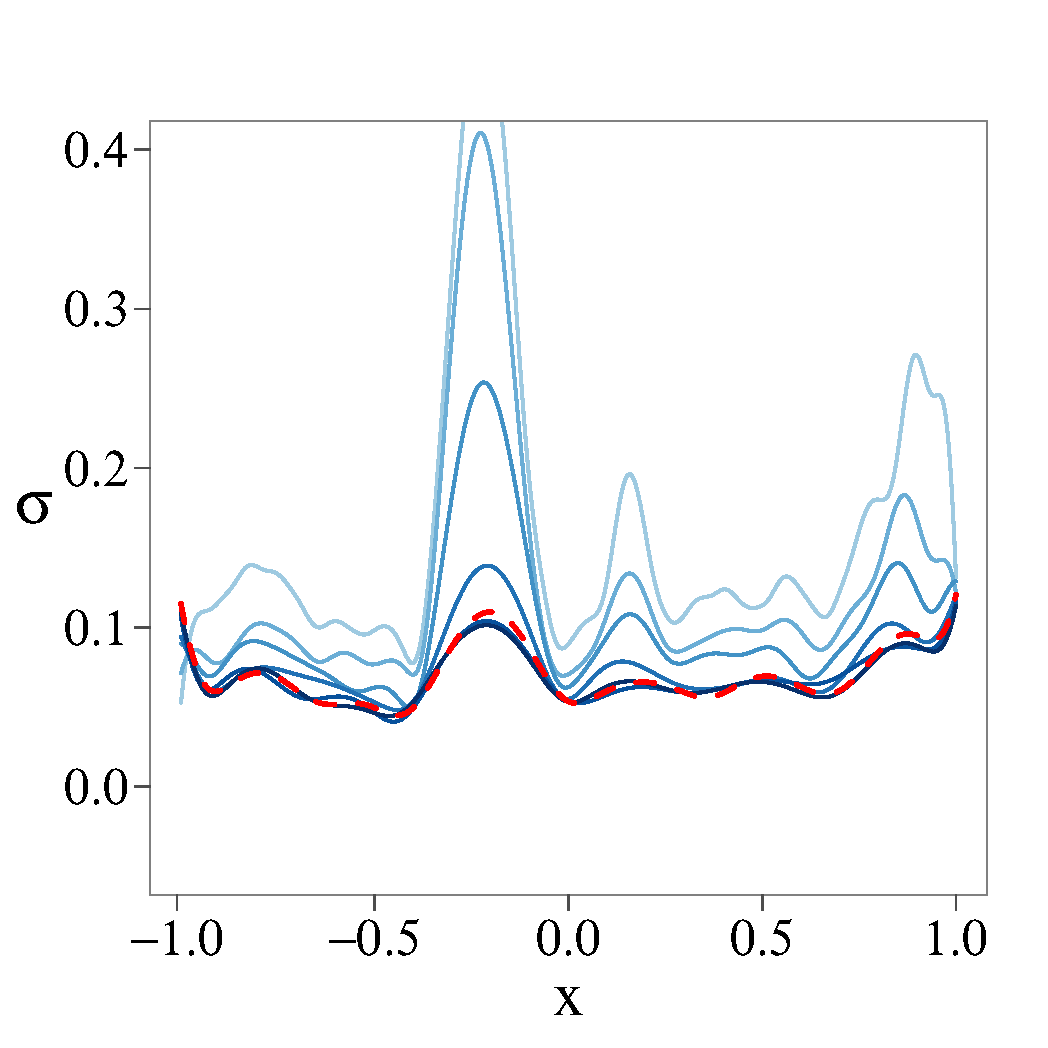
\includegraphics[scale=0.23, trim = 0mm 0mm 0mm 0mm, clip]{ch5_fig2_Sigma_L.pdf}}
\end{center}
\end{adjustwidth}

\vspace{2mm}
\begin{itemize}\setlength\itemsep{2mm}
\normalsize
\item<1-> $c$\, affects the mean mainly near the boundaries.
\item<2-> $c$\, affects the uncertainty along the whole domain and the error is greater where there is less data. 
\end{itemize}
\end{itemize}
\end{frame}
%---------------------------------------------------------------

%---------------------------------------------------------------
\begin{frame}
\setstretch{1.1}
 
\begin{itemize}\setlength\itemsep{2mm}
\item \normalsize Effect of\, $m$\, and\, $c$\\[3mm]
\begin{adjustwidth}{-4.3em}{-3em}
%
\centering
\begin{tabular}{ c c c }
\arrayrulecolor{darkgray}\hline
c = 1.05 &
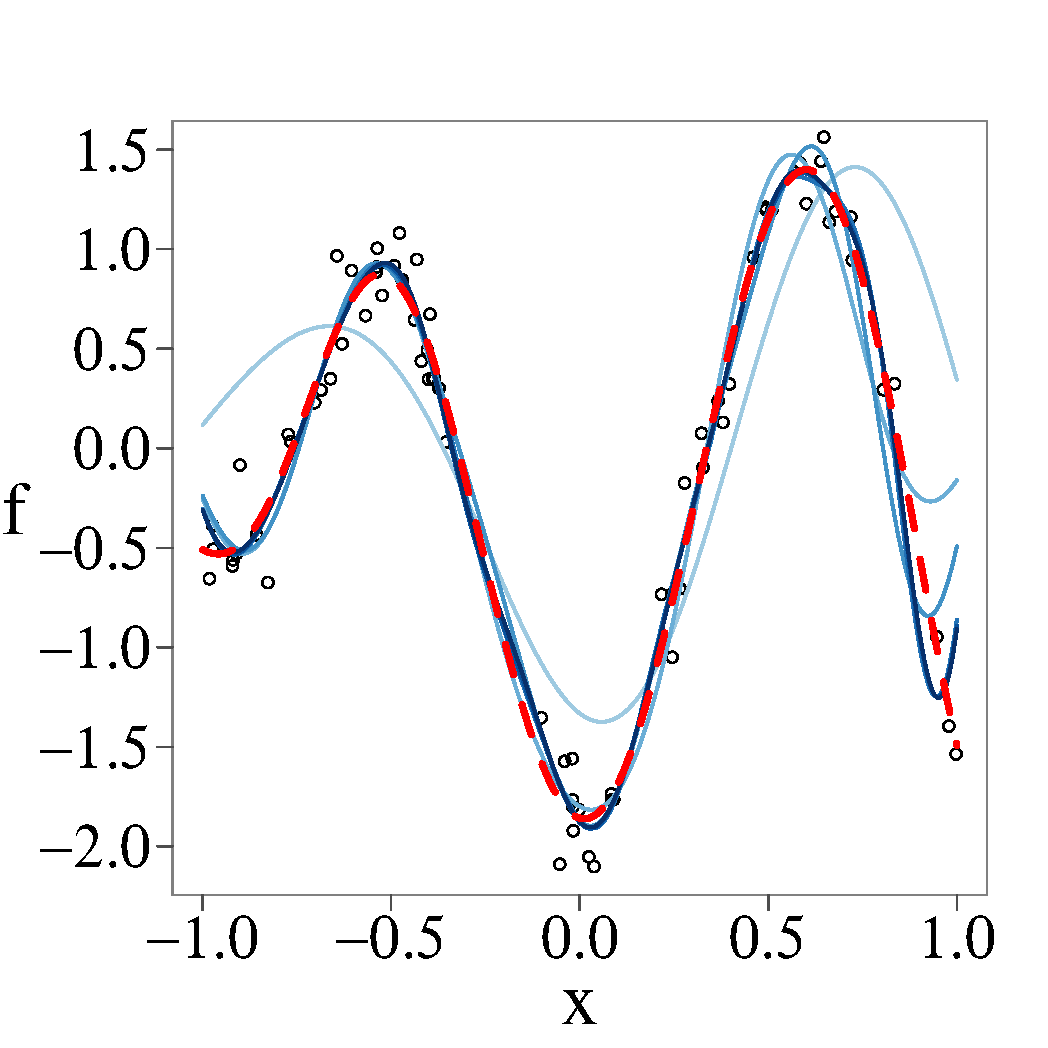
\includegraphics[scale=0.17, trim = 0mm 14mm 0mm 14mm, clip]{ch5_fig3_Post_part1.pdf}
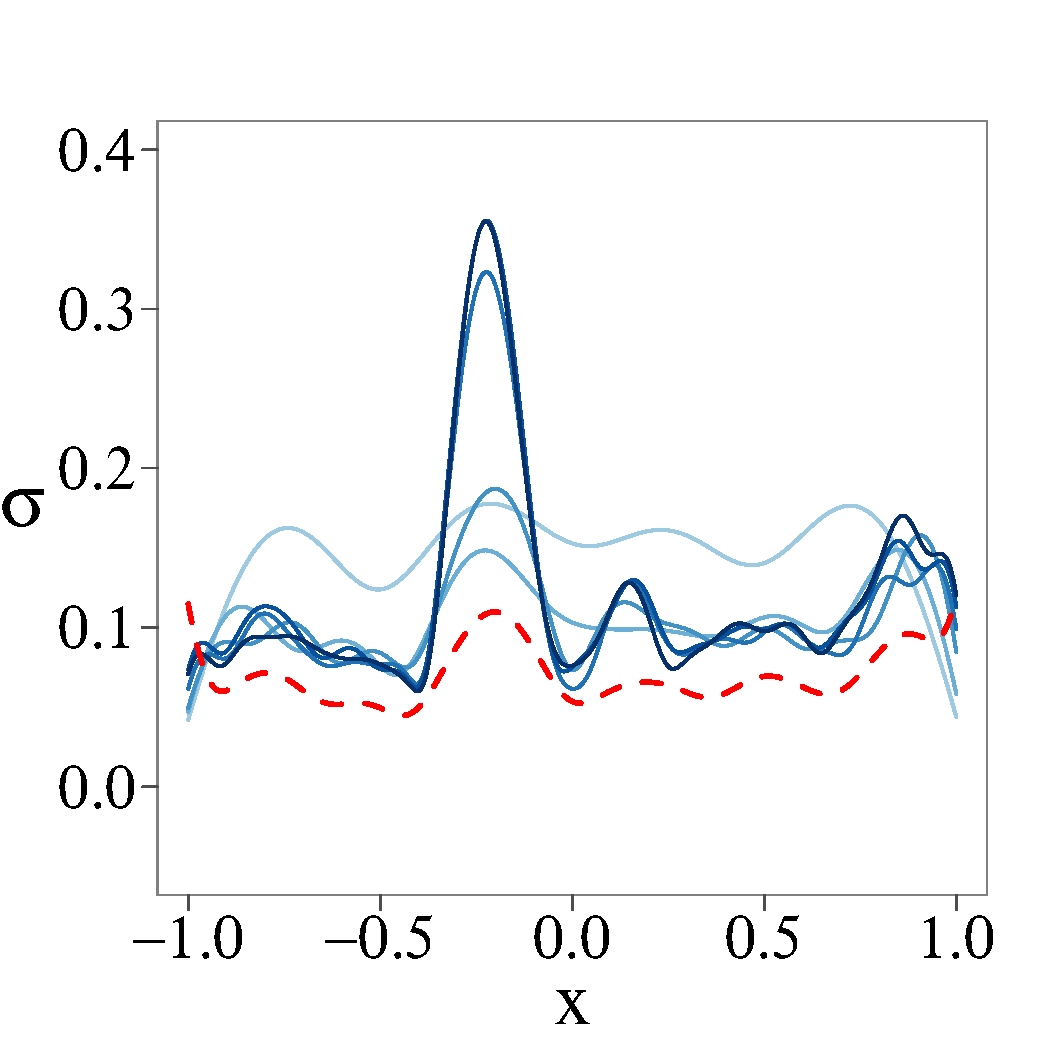
\includegraphics[scale=0.17, trim = 0mm 14mm 0mm 14mm, clip]{ch5_fig3_Sigma_part1.pdf} 
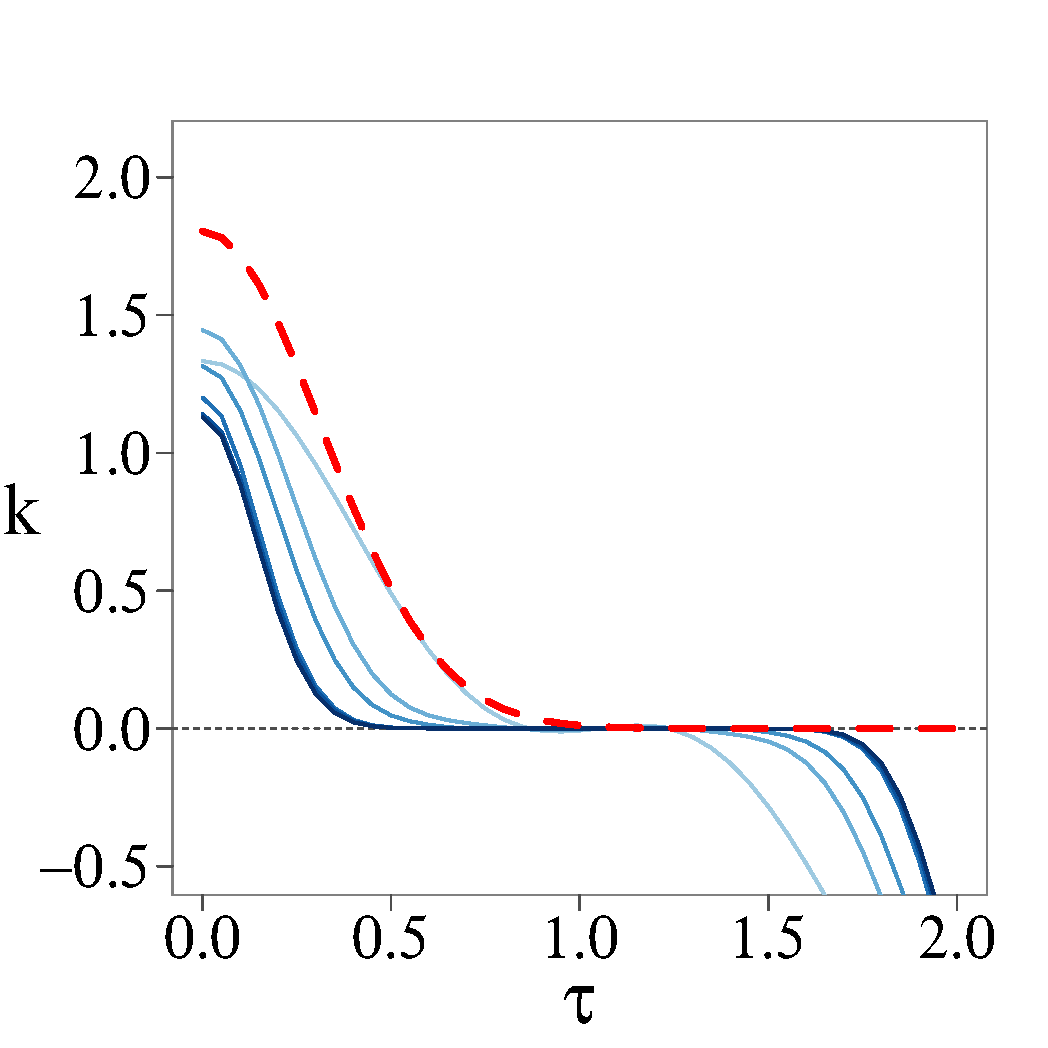
\includegraphics[scale=0.17, trim = 0mm 14mm 5mm 14mm, clip]{ch5_fig3_Cov_part1.pdf} & 
\multirow{10}{1cm}{ 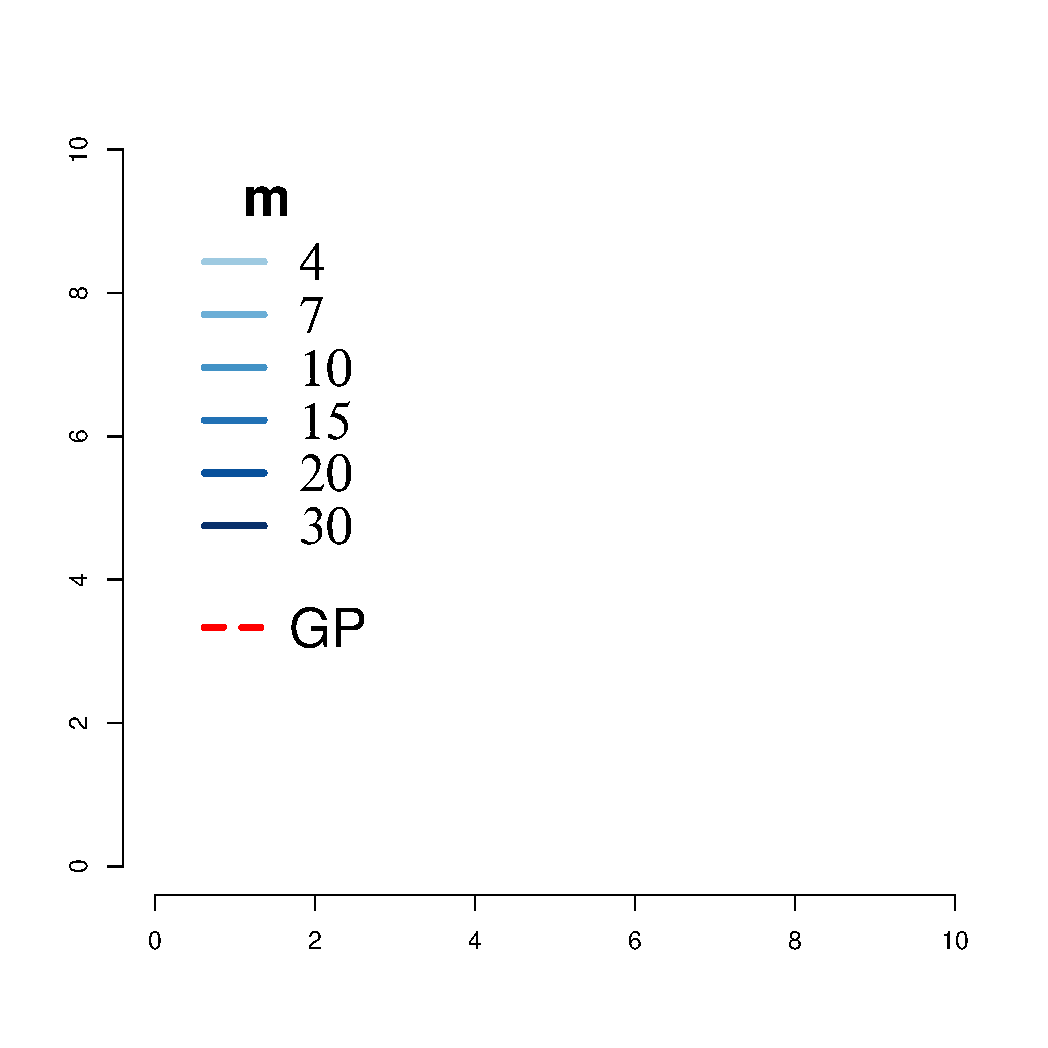
\includegraphics[scale=0.25, trim = 28mm 30mm 100mm 30mm, clip]{ch5_fig3_legend.pdf}}\\ 
\arrayrulecolor{gray!50}\hline
c = 1.1 &
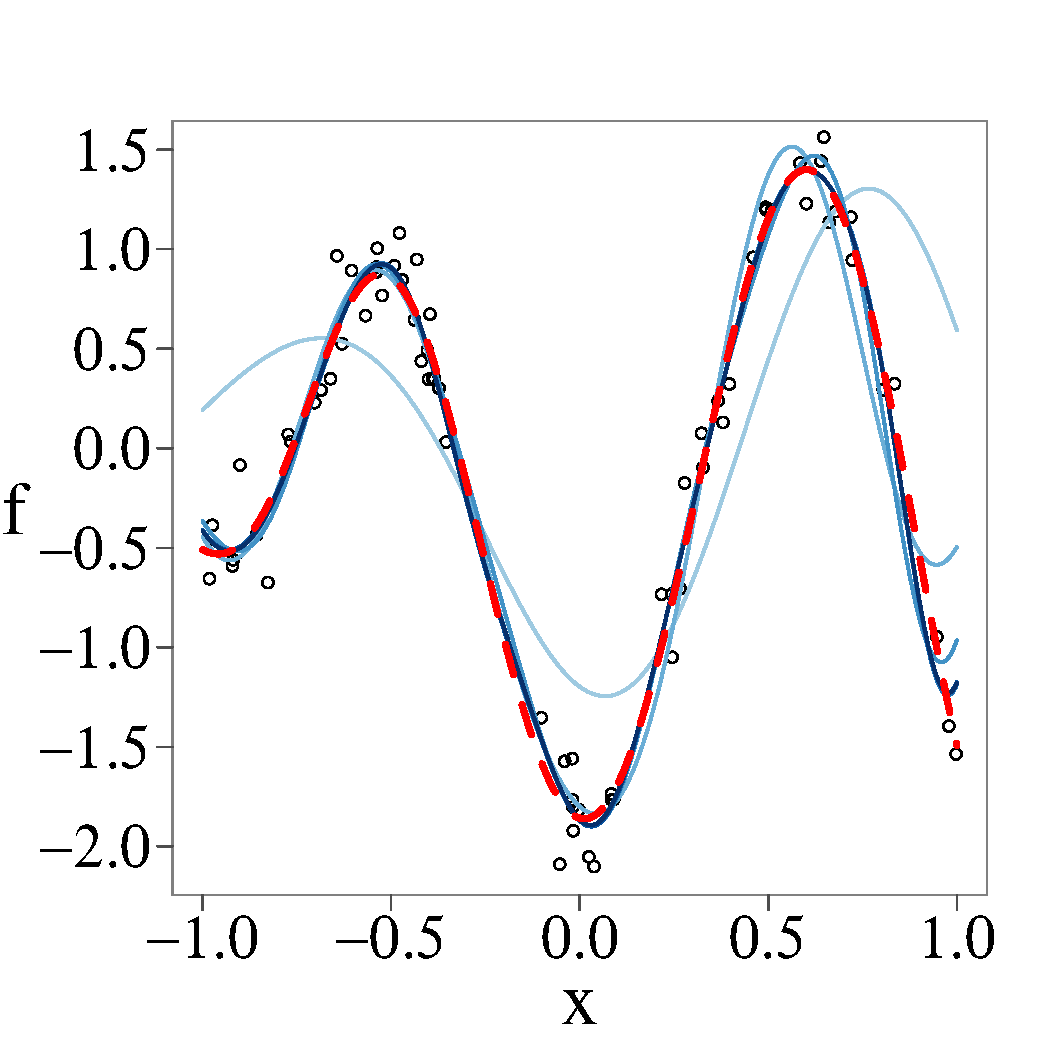
\includegraphics[scale=0.17, trim = 0mm 14mm 0mm 14mm, clip]{ch5_fig3_Post_part2.pdf} 
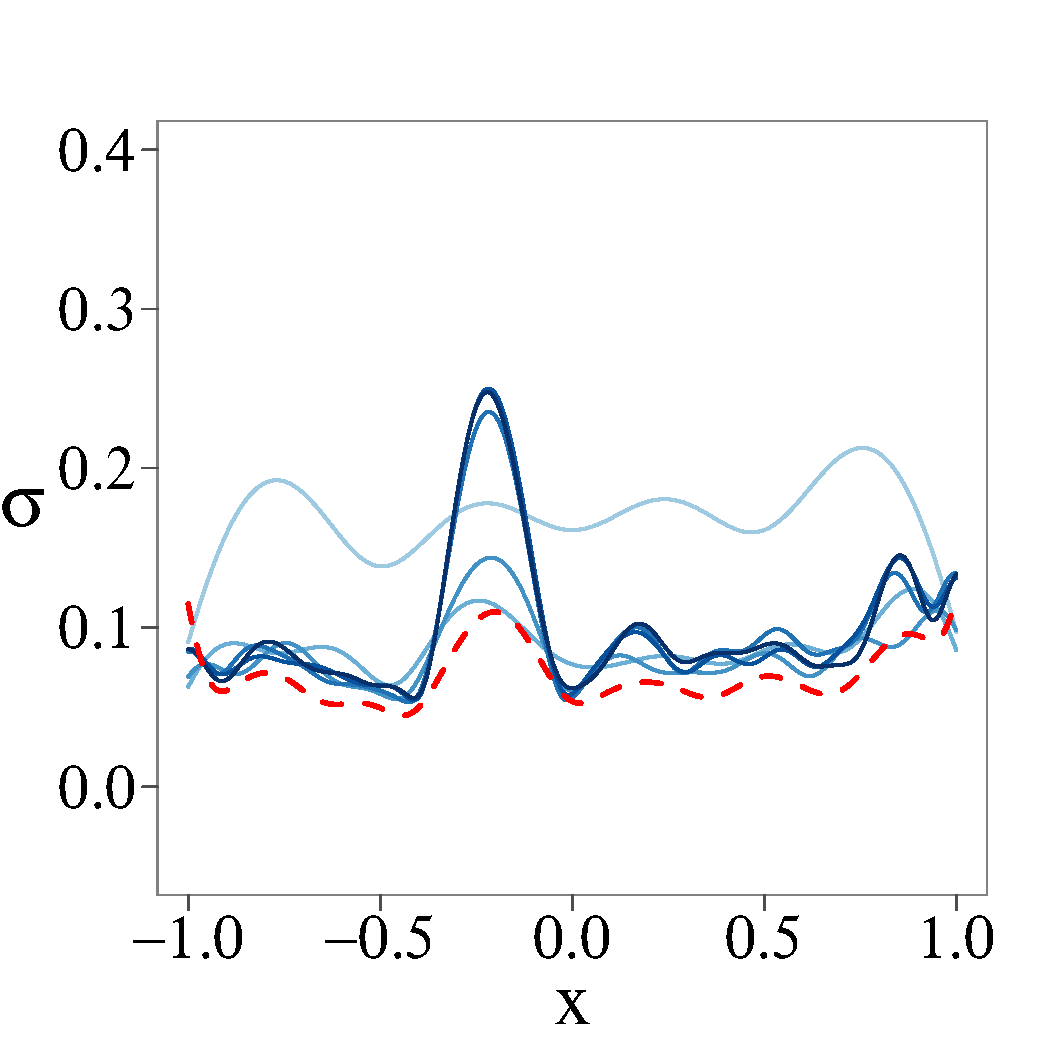
\includegraphics[scale=0.17, trim = 0mm 14mm 0mm 14mm, clip]{ch5_fig3_Sigma_part2.pdf} 
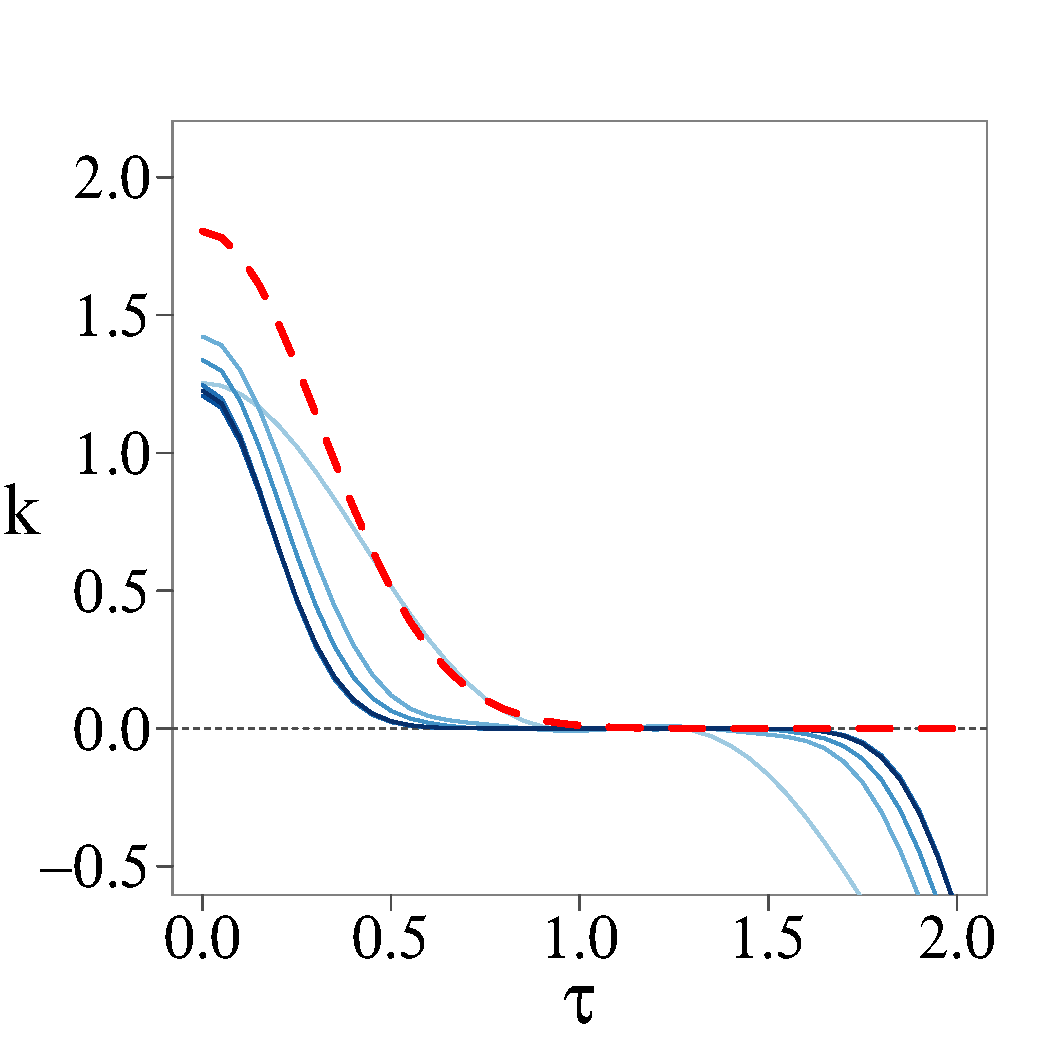
\includegraphics[scale=0.17, trim = 0mm 14mm 5mm 14mm, clip]{ch5_fig3_Cov_part2.pdf} &\\
\hline
c = 1.2 &
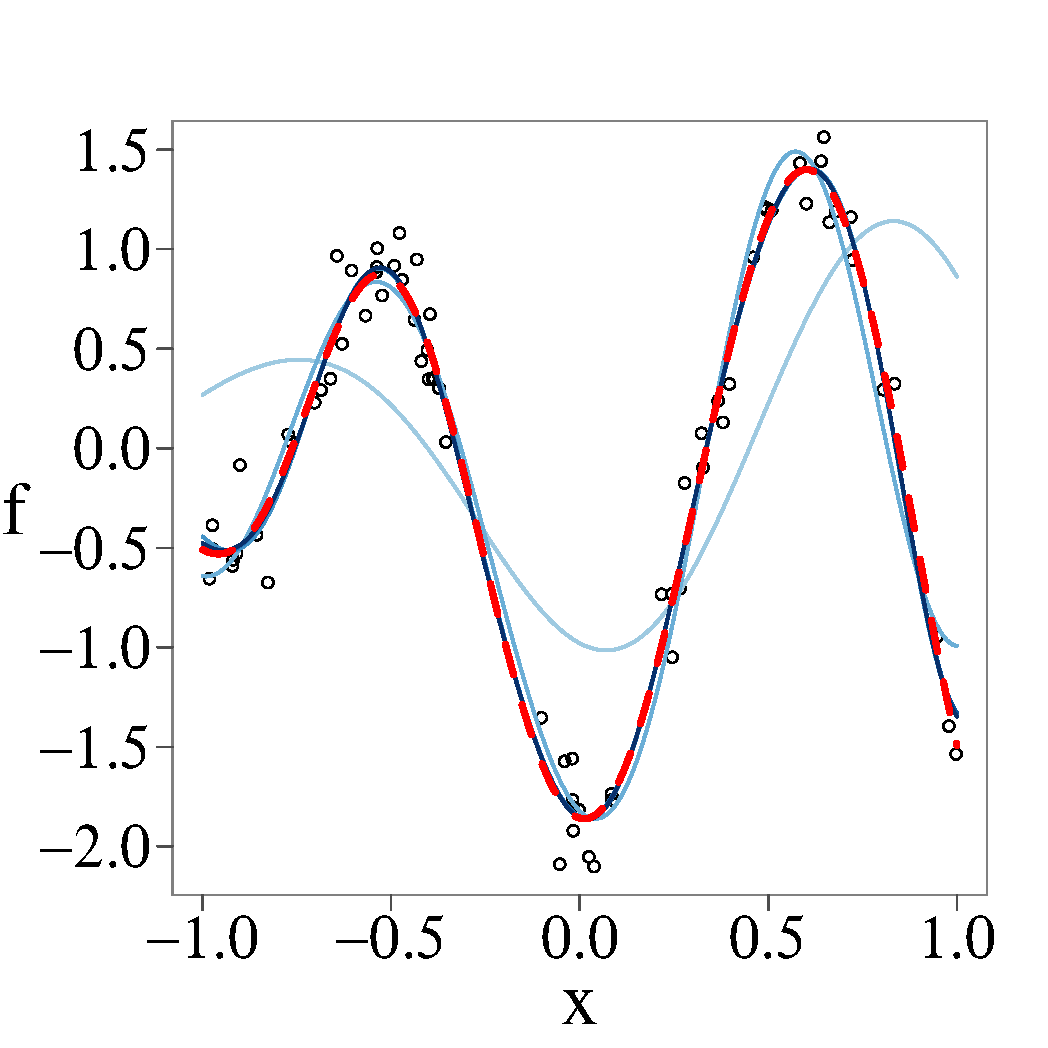
\includegraphics[scale=0.17, trim = 0mm 4mm 0mm 14mm, clip]{ch5_fig3_Post_part3.pdf} 
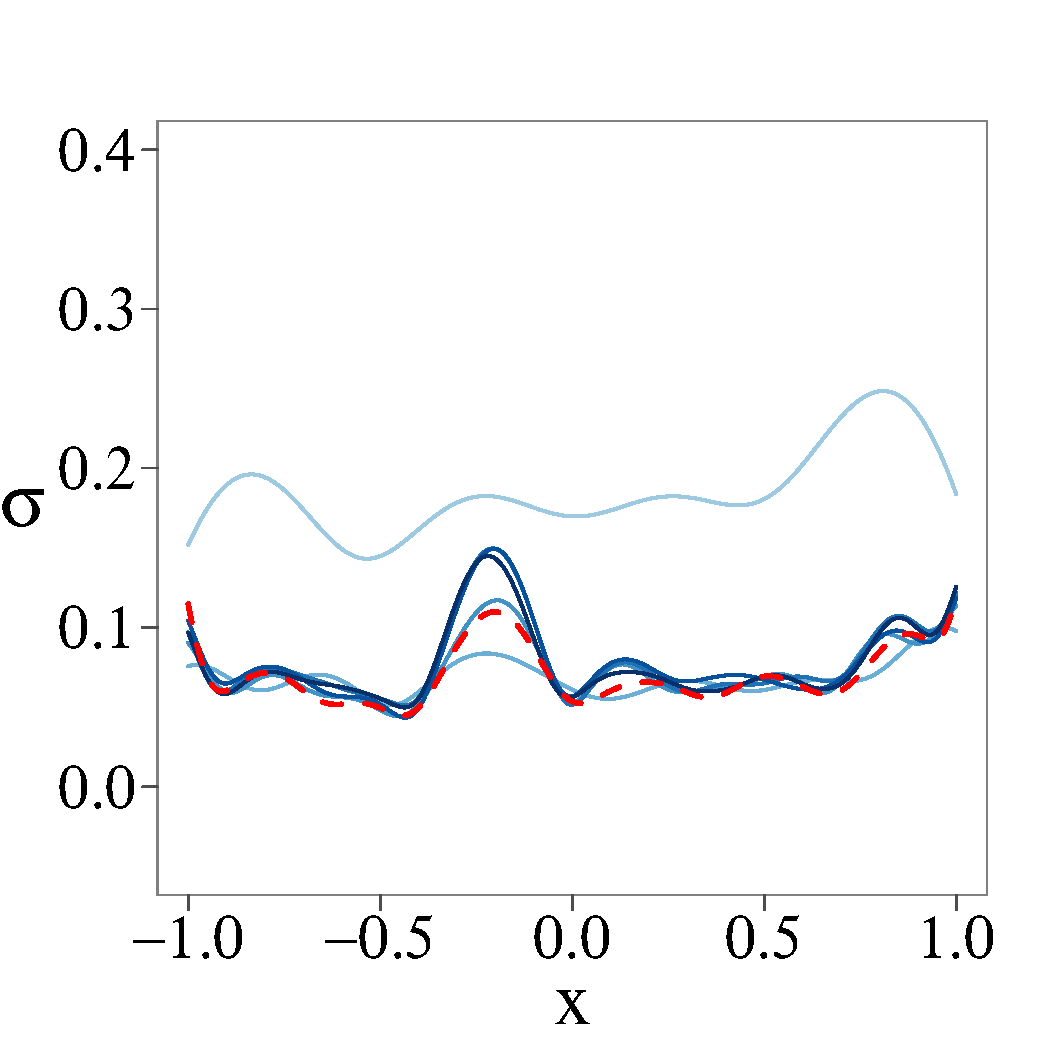
\includegraphics[scale=0.17, trim = 0mm 4mm 0mm 14mm, clip]{ch5_fig3_Sigma_part3.pdf} 
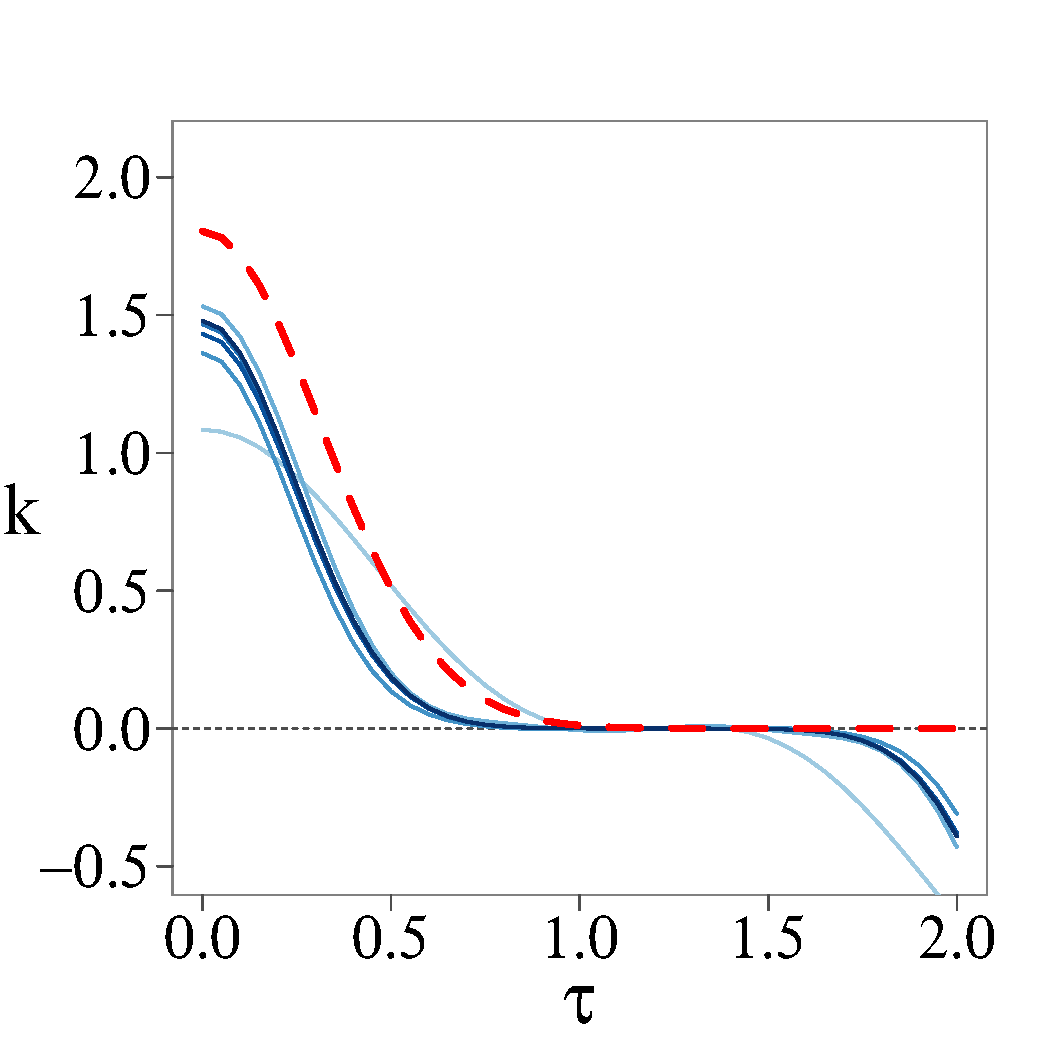
\includegraphics[scale=0.17, trim = 0mm 4mm 5mm 14mm, clip]{ch5_fig3_Cov_part3.pdf} &\\
\hline
\end{tabular}
\end{adjustwidth}
\end{itemize}
\end{frame}
%---------------------------------------------------------------

%---------------------------------------------------------------
\begin{frame}
\setstretch{1.1}
 
\begin{itemize}\setlength\itemsep{2mm}
\item \normalsize Effect of\, $m$\, and\, $c$\\[3mm]
\begin{adjustwidth}{-4.3em}{-3em}
%
\centering
\begin{tabular}{ c c c }
\arrayrulecolor{gray!50}\hline
c = 1.5 &
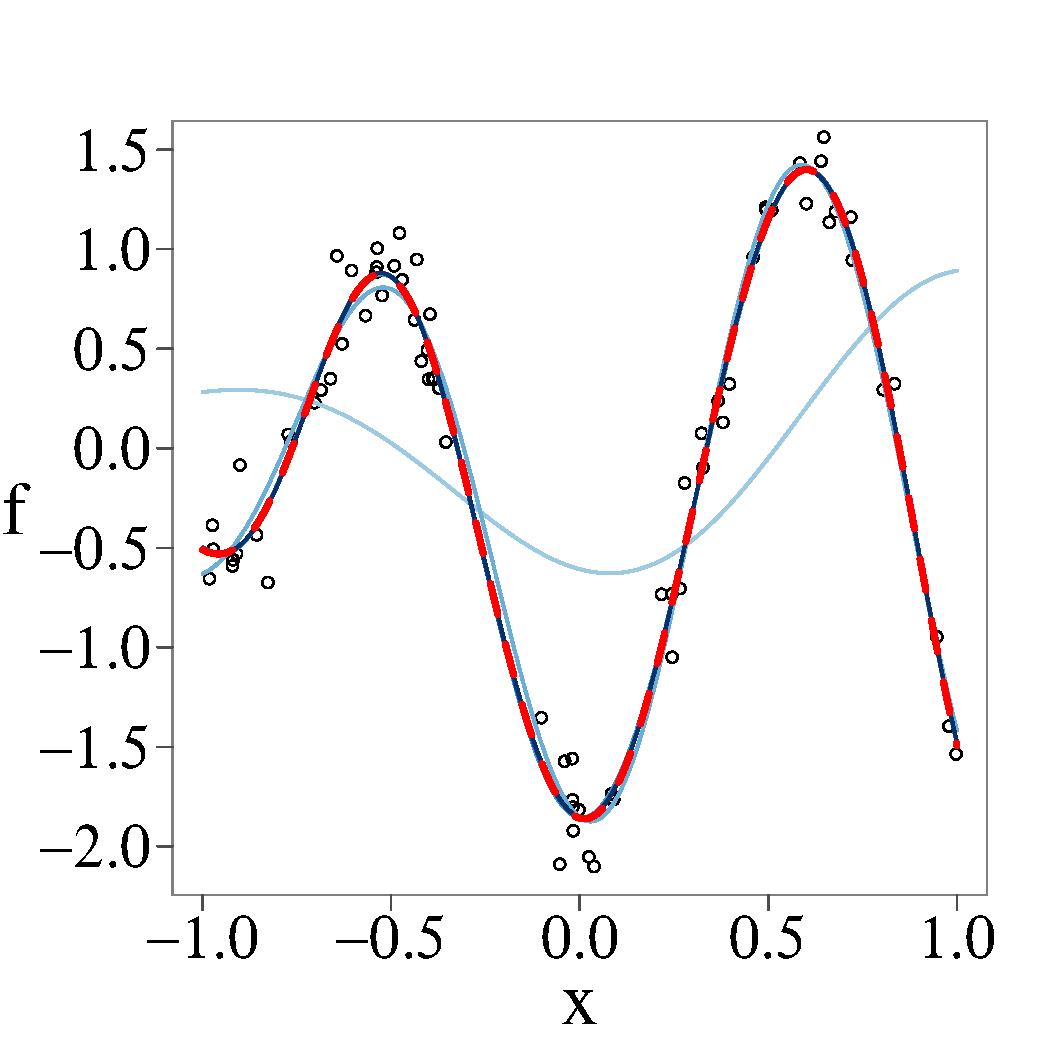
\includegraphics[scale=0.17, trim = 0mm 14mm 0mm 14mm, clip]{ch5_fig3_Post_part4.pdf} 
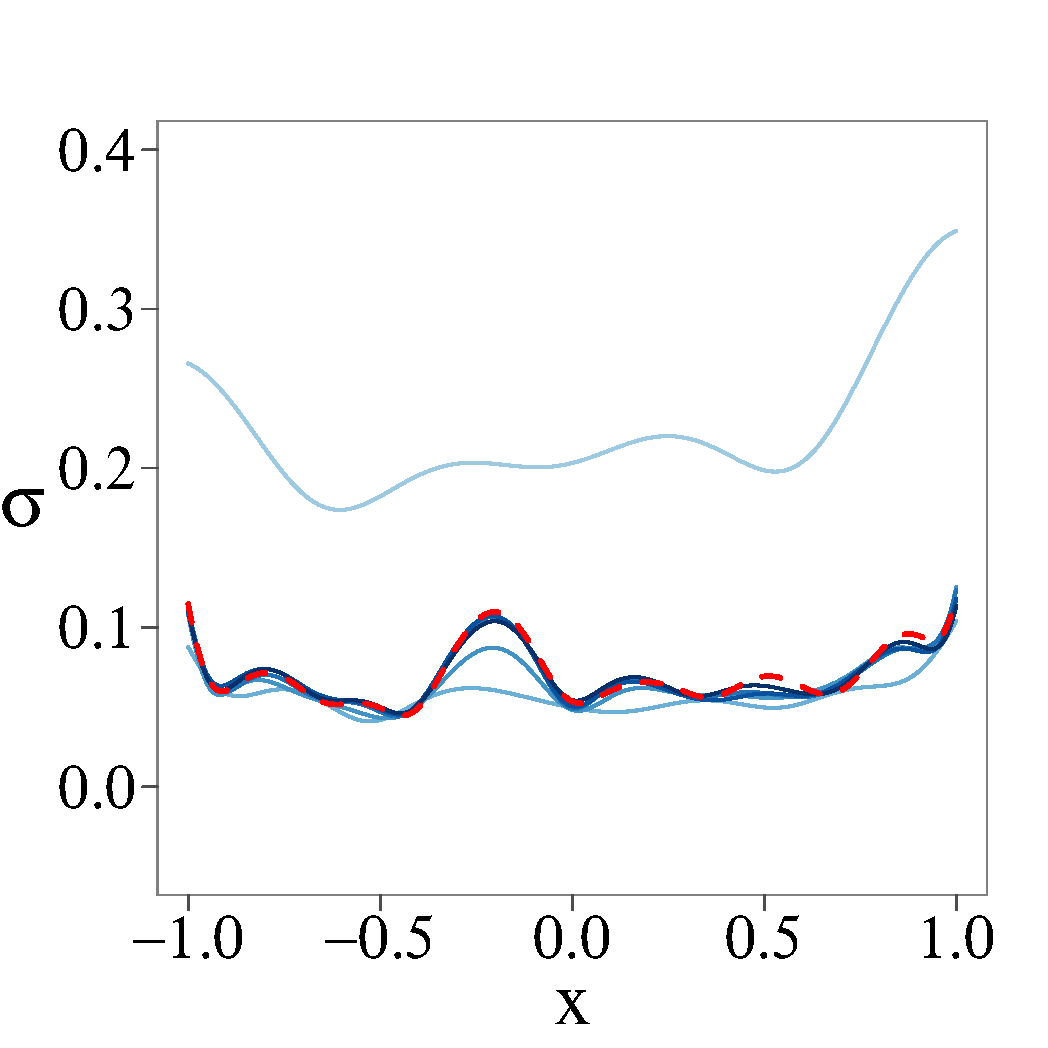
\includegraphics[scale=0.17, trim = 0mm 14mm 0mm 14mm, clip]{ch5_fig3_Sigma_part4.pdf} 
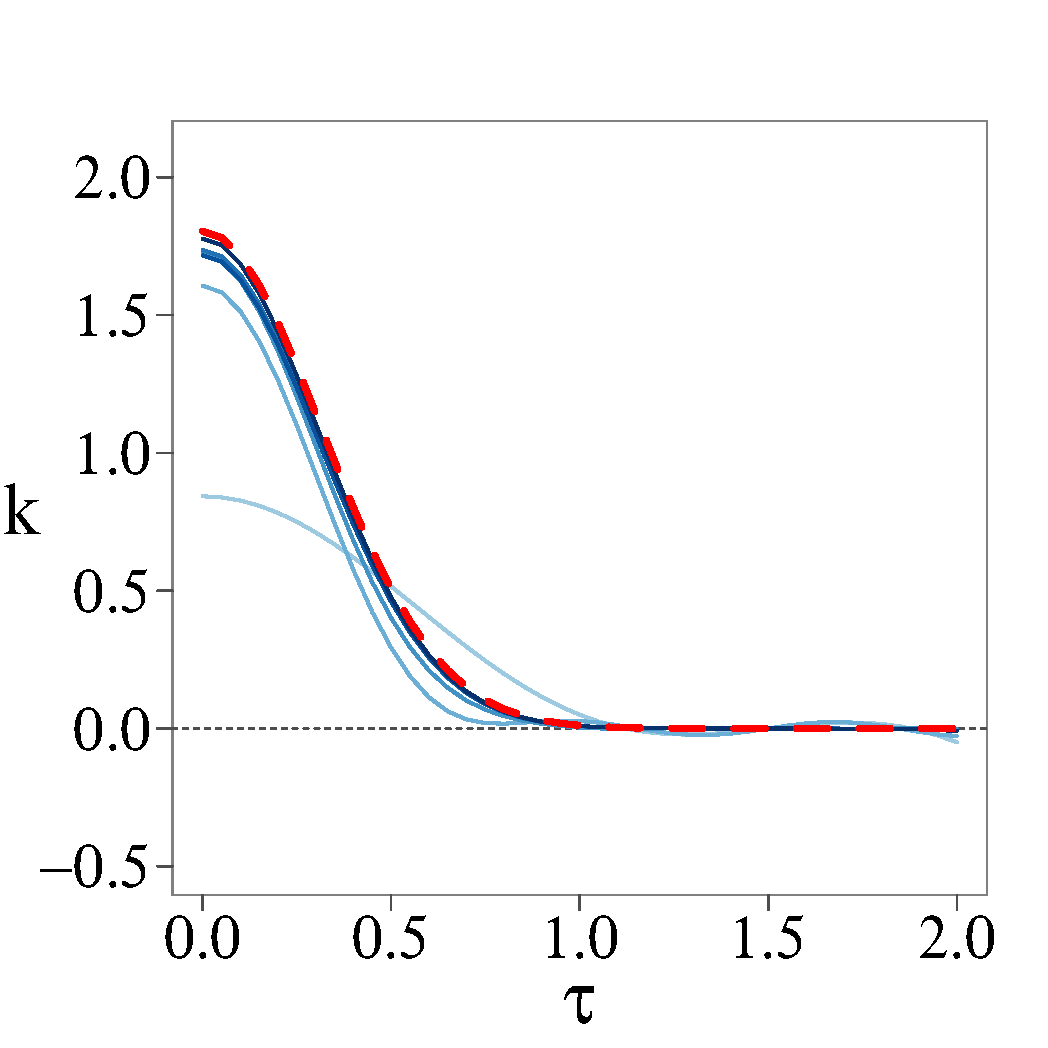
\includegraphics[scale=0.17, trim = 0mm 14mm 5mm 14mm, clip]{ch5_fig3_Cov_part4.pdf} & 
\multirow{10}{1cm}{ 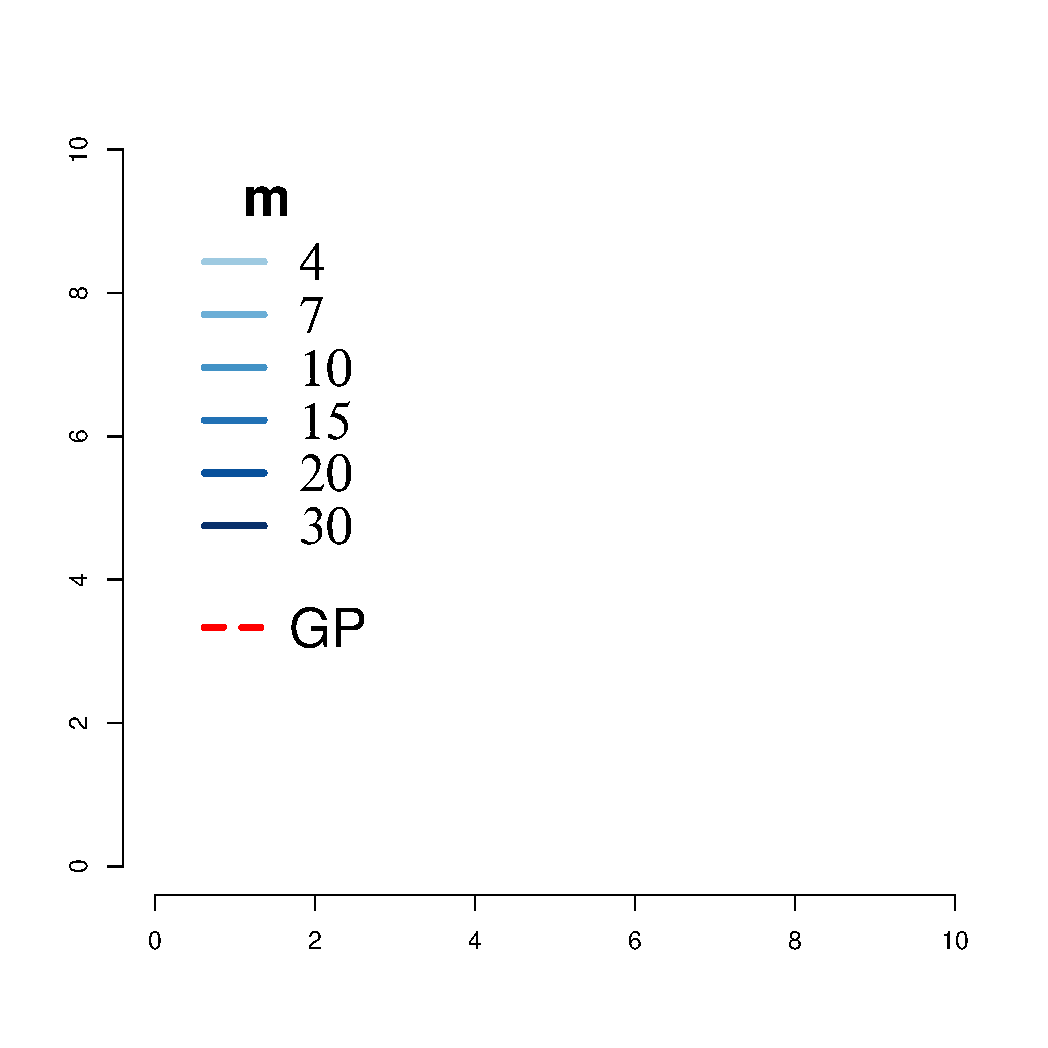
\includegraphics[scale=0.25, trim = 28mm 30mm 100mm 30mm, clip]{ch5_fig3_legend.pdf}}\\
\hline
c = 2 &
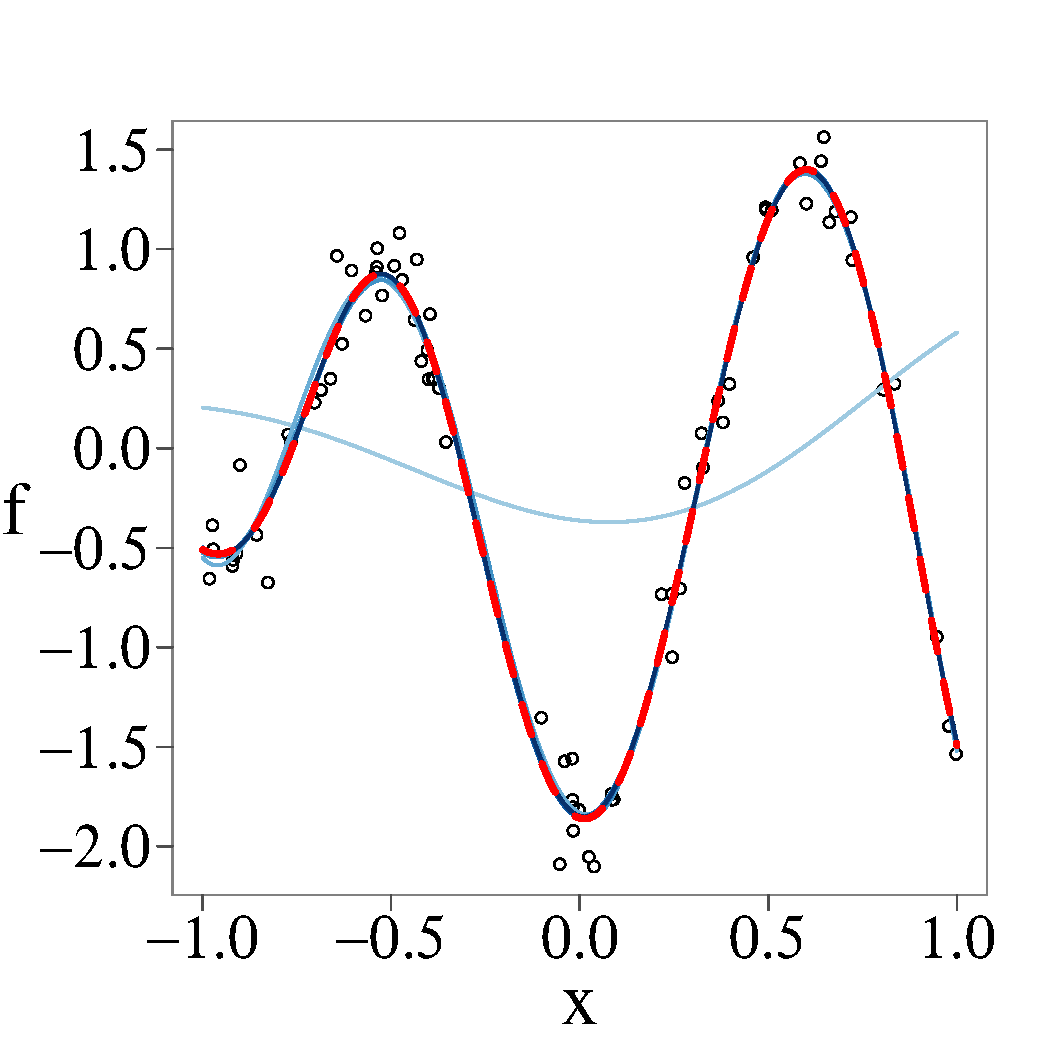
\includegraphics[scale=0.17, trim = 0mm 14mm 0mm 14mm, clip]{ch5_fig3_Post_part5.pdf} 
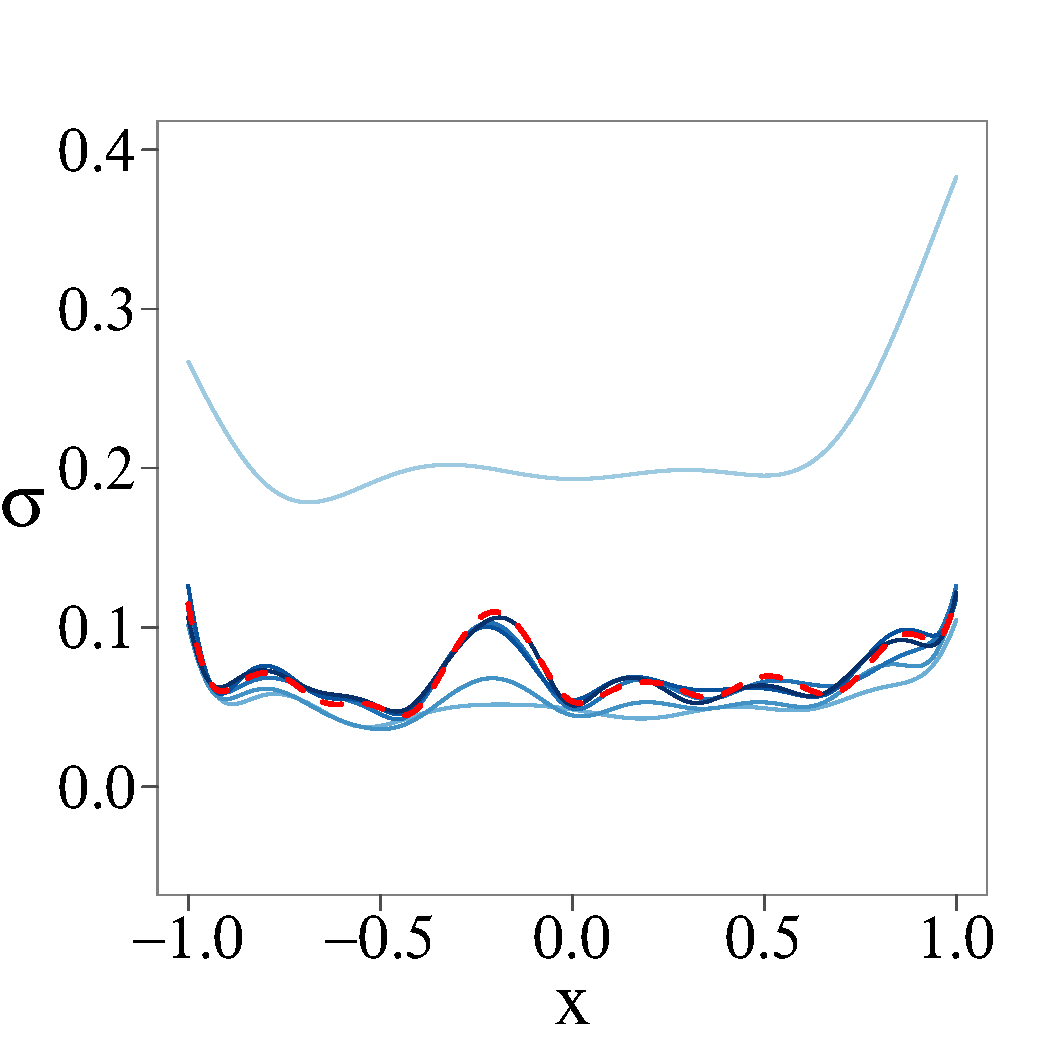
\includegraphics[scale=0.17, trim = 0mm 14mm 0mm 14mm, clip]{ch5_fig3_Sigma_part5.pdf} 
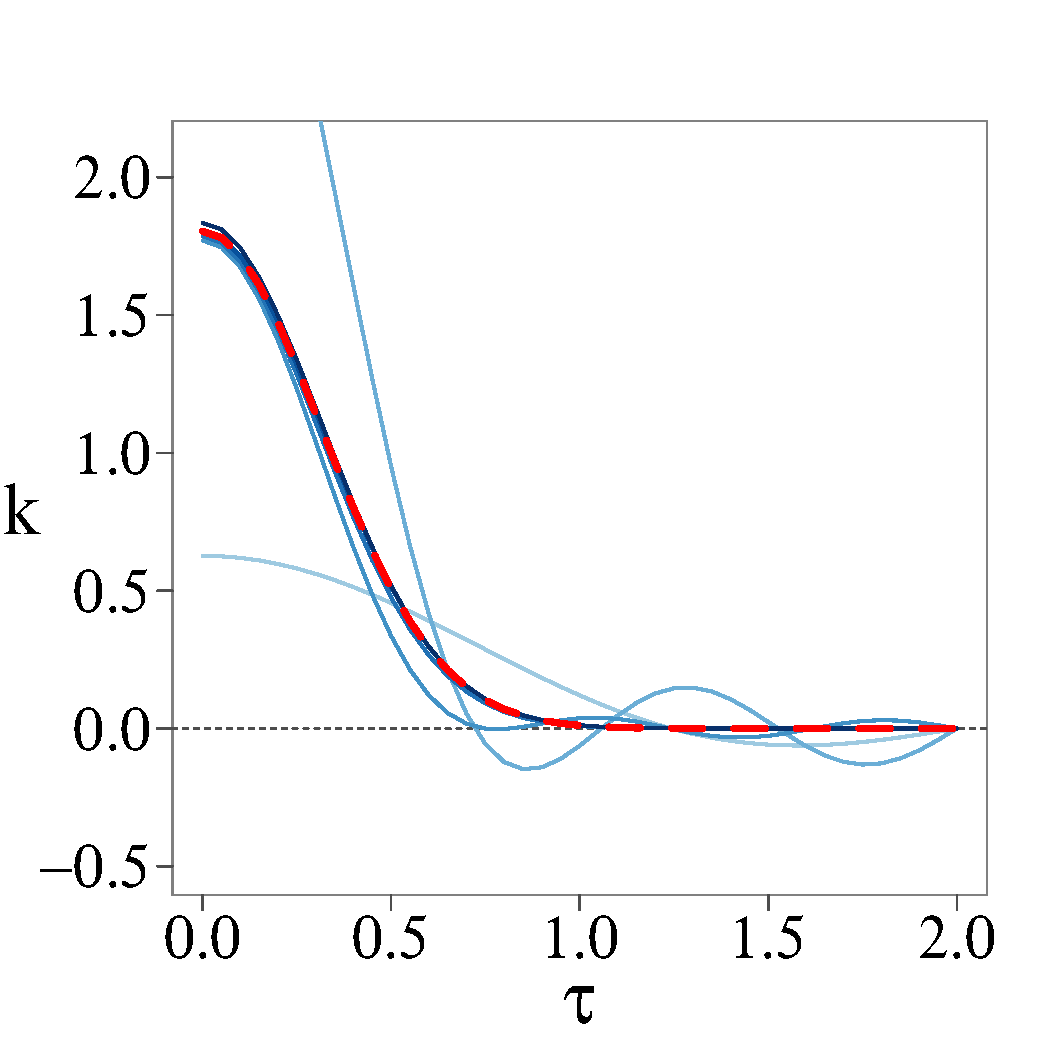
\includegraphics[scale=0.17, trim = 0mm 14mm 5mm 14mm, clip]{ch5_fig3_Cov_part5.pdf} & \\
\hline
c = 2.5 &
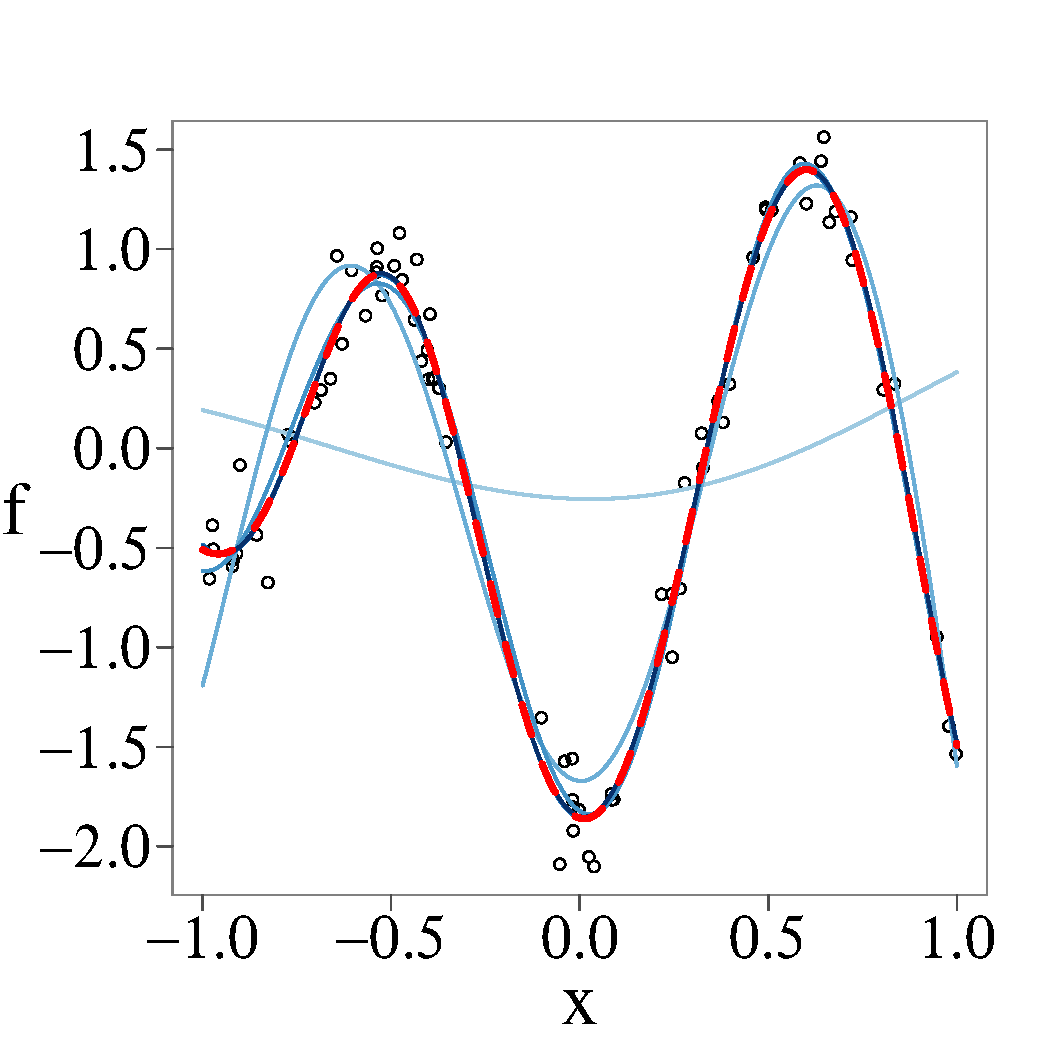
\includegraphics[scale=0.17, trim = 0mm 4mm 0mm 14mm, clip]{ch5_fig3_Post_part6.pdf}
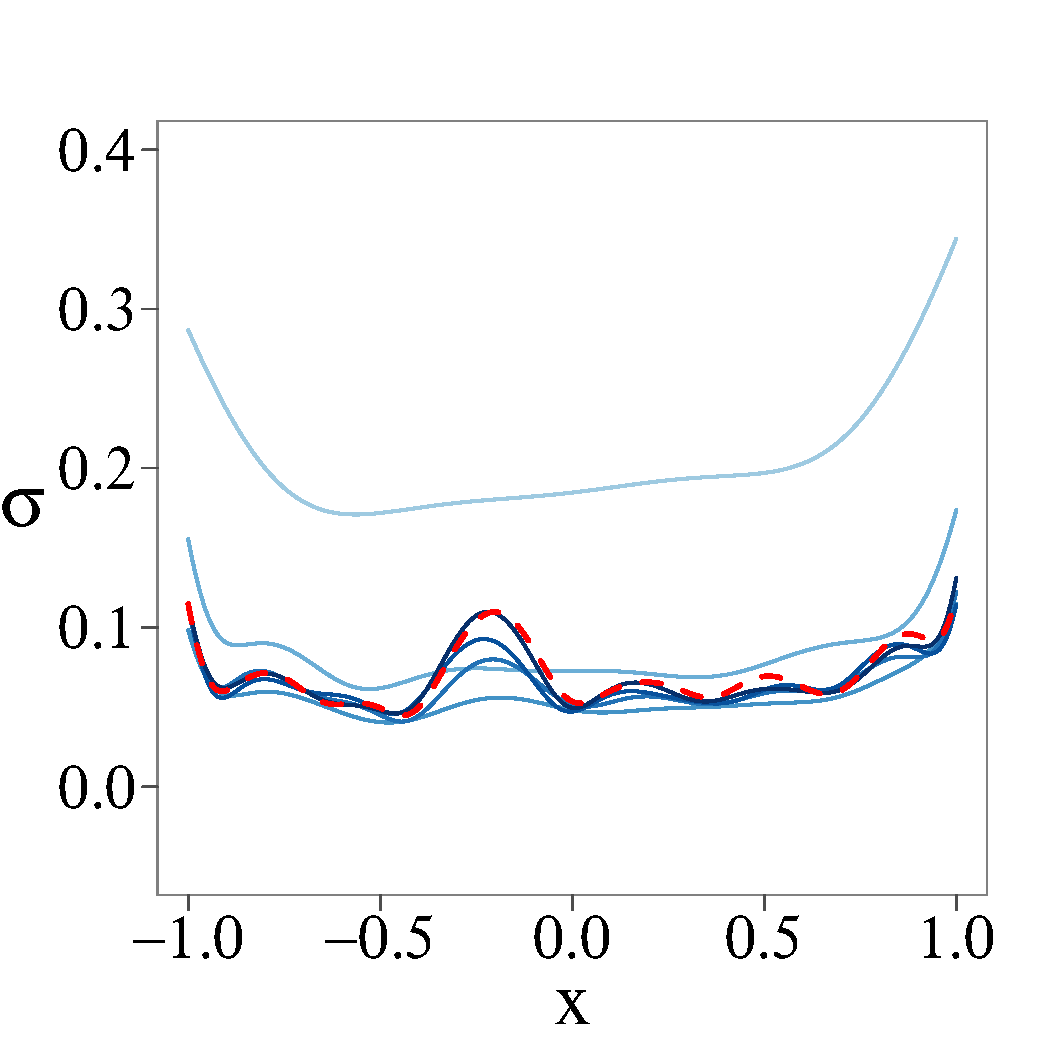
\includegraphics[scale=0.17, trim = 0mm 4mm 0mm 14mm, clip]{ch5_fig3_Sigma_part6.pdf}
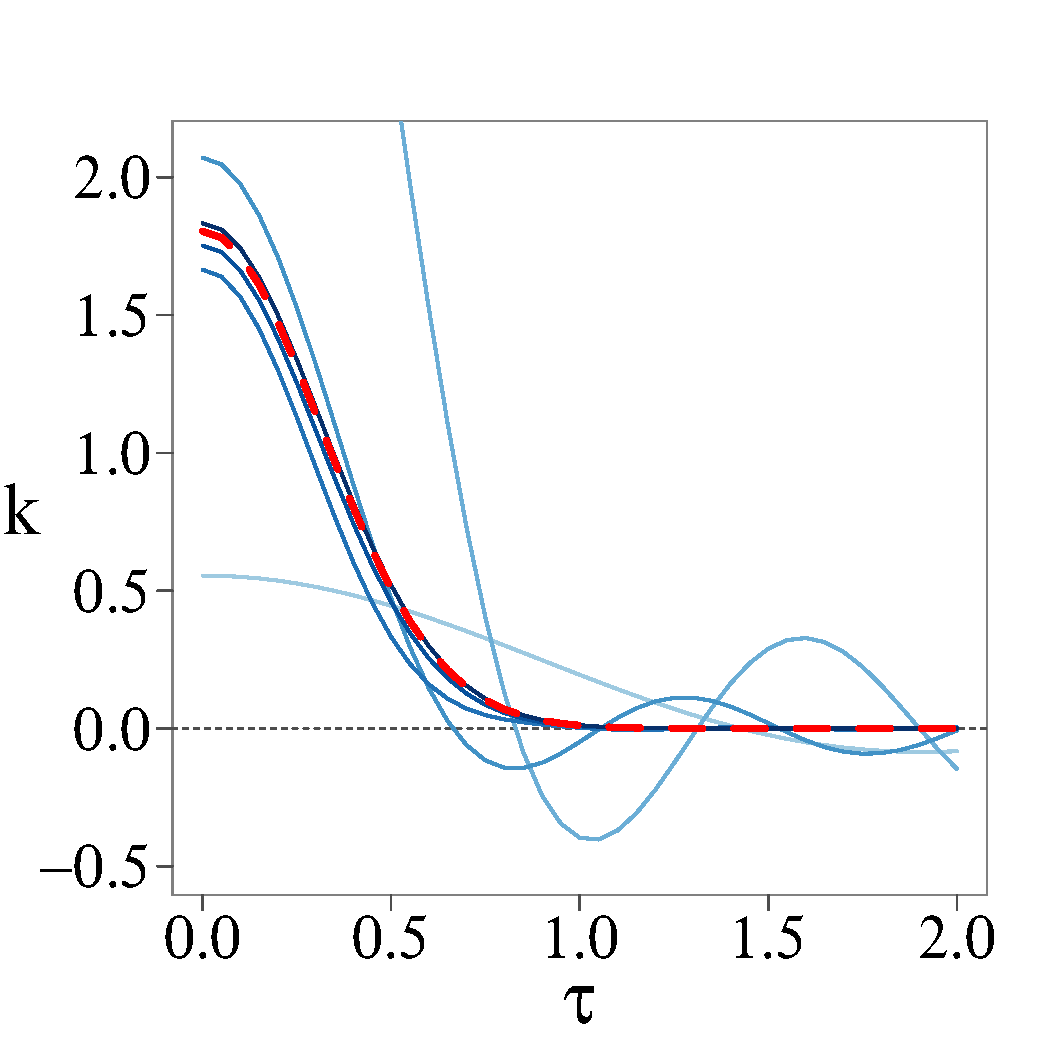
\includegraphics[scale=0.17, trim = 0mm 4mm 5mm 14mm, clip]{ch5_fig3_Cov_part6.pdf} &\\
\arrayrulecolor{darkgray}\hline
\end{tabular}
\end{adjustwidth}
\end{itemize}
\end{frame}
%---------------------------------------------------------------

%---------------------------------------------------------------
\begin{frame}[t]
\setstretch{1.1}

\vspace{-3mm}
\begin{adjustwidth}{-0.5em}{-2em}
\only<1>{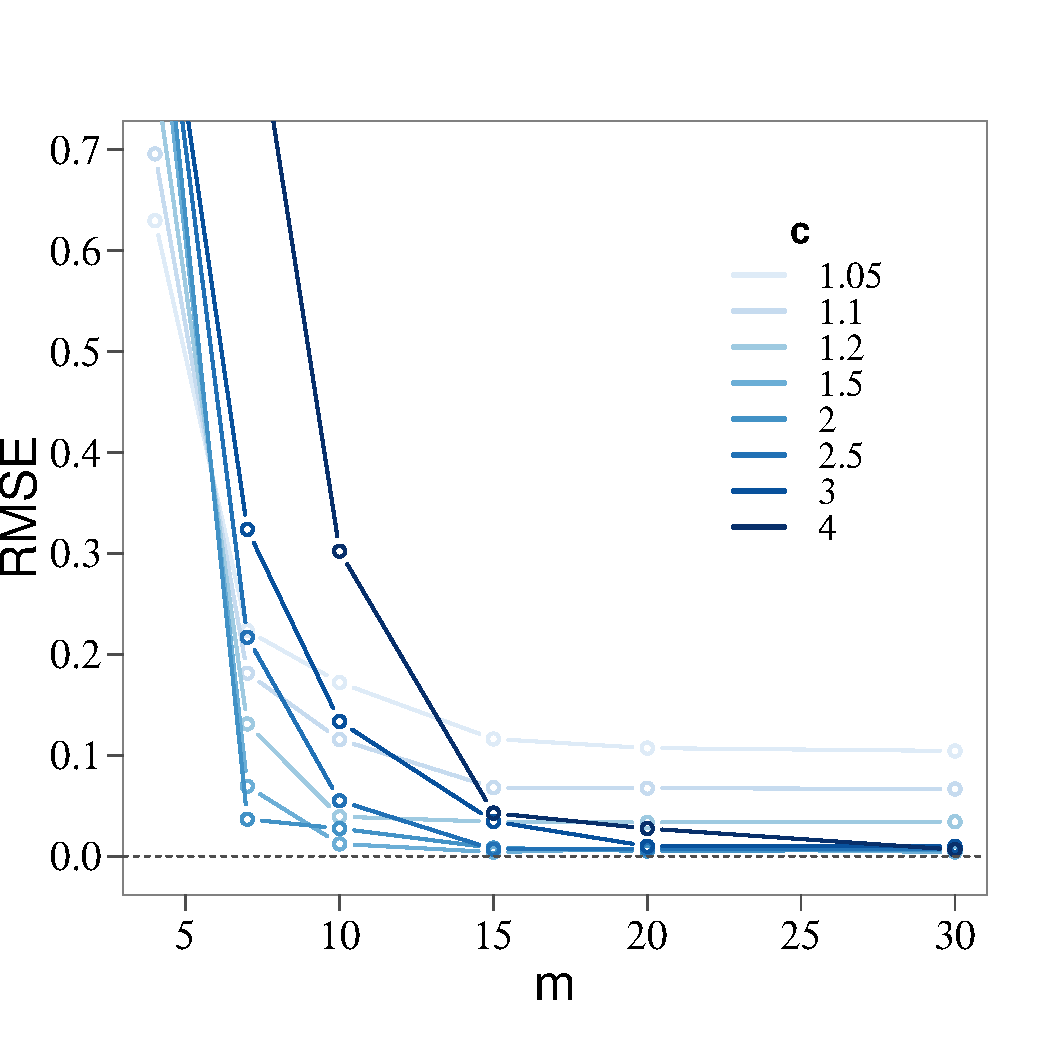
\includegraphics[scale=0.34, trim = 0mm 8mm 0mm 0mm, clip]{ch5_fig4_MSE_vs_J.pdf} }
\only<2>{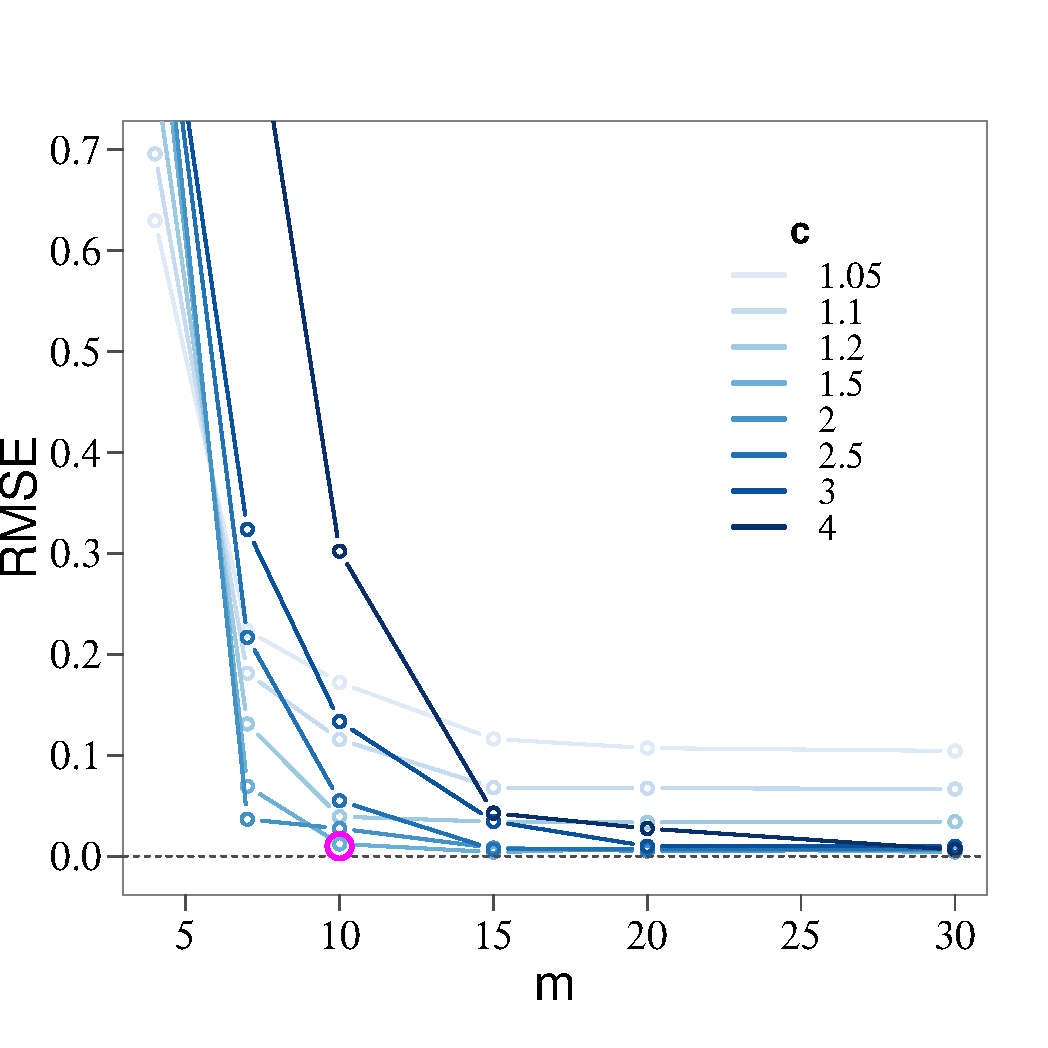
\includegraphics[scale=0.34, trim = 0mm 8mm 0mm 0mm, clip]{performance_fig1.pdf} }
\only<3>{\includegraphics[scale=0.34, trim = 0mm 8mm 0mm 0mm, clip]{performance_fig2.pdf} }
\only<4-5>{\includegraphics[scale=0.34, trim = 0mm 8mm 0mm 0mm, clip]{performance_fig3.pdf} }
%
\visible<5->{\includegraphics[scale=0.35, trim = 0mm 8mm 10mm 0mm, clip]{ch5_fig5_lscale_vs_J.pdf}}
\end{adjustwidth}

\centering
\begin{tcolorbox}[colframe=blue!20, colback=white, title={\small Main conclusions}, colbacktitle=lightblue, coltitle=black, boxrule=0.5pt, right=1mm, left=1mm, width=0.99\textwidth]
\setstretch{1.1}
\begin{itemize}
\item \; As\, $c$\, increases,\, $m$ has to increase as well (and vice versa). 
$$
\small
\text{As}\;\, L=c\cdot S,\hspace{3mm} \text{if}\; c\uparrow,\; \text{then}\; \lambda_j=\left(\frac{j\pi}{2L}\right)^{\!2}\downarrow,\, \text{and therefore}\;\, S_{\theta}(\sqrt{\lambda_j})\downarrow \; \text{and}\; m\; \downarrow
$$ 
\item \; There exists a minimum valid\, $c$,\, regardless\, $m$. % below which a accurate approximation will never be achieved.
\end{itemize}
\end{tcolorbox}
\end{frame}
%---------------------------------------------------------------


\subsection*{Model of relationships among $m$, $L$ and $\ell$}
%---------------------------------------------------------------
\begin{frame}
\setstretch{1.1}

\begin{enumerate}\setcounter{enumi}{1}
\item \textbf{Model of relationships among}\, $m$,\, $c$\, \textbf{and}\, $\ell$ \\[2mm]

 \begin{itemize}
 \item make useful and valuable {\color{navyblue} recomendations} 
 \item make {\color{navyblue} diagnosis} of the performance 
 \item save time of computation 
 \end{itemize}
\end{enumerate}

\vspace{3mm}
\begin{columns}
\column{0.2\textwidth}

\column{0.4\textwidth}
\hspace{5mm} \centering \scriptsize Squared exponential kernel\\
\includegraphics[scale=0.25, trim = 0mm 0mm 5mm 10mm, clip]{ch5_fig6_lscale_vs_J_vs_c_zoomin.pdf}

\column{0.6\textwidth}
\begin{itemize}
\scriptsize
\item[] $m$\, and $c$\, govern the approximation.\\
\item[] $\ell$\, controls the wigglyness of the function.
\end{itemize}

\begin{columns}
\column{5mm}
 \includegraphics[scale=0.25, trim = 80mm 110mm 210mm 40mm, clip]{performance_fig4.pdf}
\column{40mm}
 \pbox{4cm}{\scriptsize in terms of an accurate approximation}
\column{5mm}
\end{columns}
\end{columns}

\centering
\begin{tcolorbox}[colframe=blue!20, colback=white, title={\scriptsize Criteria of an accurate approximation as a function of $m$}, colbacktitle=lightblue, coltitle=black, boxrule=0.5pt, width=0.8\textwidth]
\setstretch{1.1}
\scriptsize
{\small Relative difference among approximate and exact covariance:}
%
\begin{align*}
 \int \frac{ | k(\tau) - \sum_{j=1}^m S_{\theta}(\sqrt{\lambda_j}) \phi_j(\tau) \phi_j(0)|}{k(\tau)} \,\mathrm{d}\tau < 0.01
\end{align*}
\end{tcolorbox}
\end{frame}
%---------------------------------------------------------------

%---------------------------------------------------------------
\begin{frame}
\setstretch{1.1}

\vspace{3mm}

\begin{columns}
\column{0.4\textwidth}
\hspace{7mm} \centering \scriptsize Squared exponential\\
\includegraphics[scale=0.29, trim = 0mm 0mm 5mm 10mm, clip]{ch5_fig6_lscale_vs_J_vs_c_zoomin.pdf}

\column{0.5\textwidth}
\hspace{7mm} \centering \scriptsize Mattern($\nu$=3/2) kernel\\
\includegraphics[scale=0.29, trim = 0mm 0mm 5mm 10mm, clip]{ch5_fig6_lscale_vs_J_vs_c_zoomin_Matern.pdf}
\end{columns}

\begin{tcolorbox}[colframe=blue!20, colback=white, title={\small This model says...}, colbacktitle=lightblue, coltitle=black, boxrule=0.5pt]
\setstretch{1.1}
\begin{itemize}\setlength\itemsep{1mm}
\item For a given\, $m$\, and\, $c$,\, the minimum\, $\ell$\, that can be accurately approximated.
\item For a given\, $\ell$\, and\, $c$,\, the minimum\, $m$\, required for an accurate approximation.
\item For a given\, $\ell$\, and\, $m$,\, the highest\, $c$\, allowed for an accurate approximation.
\item The minimum valid\, $c$\, for a given\, $\ell$.
\end{itemize}
\end{tcolorbox}

\end{frame}
%---------------------------------------------------------------

%---------------------------------------------------------------
\begin{frame}
\setstretch{1.1}

\begin{tcolorbox}[colframe=blue!20, colback=white, title={\small Insights from this model of relationships}, colbacktitle=lightblue, coltitle=black, boxrule=0.5pt]

\begin{itemize}\setlength\itemsep{1mm}
\item Allows to  choose the combination ($m,c$) that accurately approximate\, $\ell$\, and save computation time.\\[-5mm]
$$
O(nm+m)
$$

\item Serves as a {\color{navyblue} diagnosis tool} of the approximation:

\begin{remark}
\setstretch{1.1}
As the lengthscale is the parameter that ultimately characterizes the non-linearity of the posterior functions, we assume we can look at the {\color{navyblue} estimate lengthscale} to diagnose the approximation.
\end{remark}

\vspace{2mm}
\item Given $m$ and $c$

\item If\, $\hat{\ell}$\, {\color{navyblue} is below} the minimum\, $\ell$\, that can be accurately approximated (for those given\, $m$\, and\, $c$), then the approximation {\color{navyblue} is not sufficiently accurate}, and\, $m$\, must be increased or\, $c$\, decreased.

\item If\, $\hat{\ell}$\, {\color{navyblue} is above} the minimum\, $\ell$, then the approximation should be {\color{navyblue} sufficiently accurate}.

\item This can be done iteratively.

%\item $c$\, can not be decreased as much as desired because it is restricted to\, $\ell$.
\end{itemize}
\end{tcolorbox}
\end{frame}
%---------------------------------------------------------------

%---------------------------------------------------------------
\begin{frame}
\setstretch{1.1}

\textsc{\small Example of diagnosis}\\

\vspace{-4mm}
\centering
\includegraphics[scale=0.25, trim = 0mm 8mm 0mm 0mm, clip]{ch5_fig4_MSE_vs_J.pdf}

\vspace{2mm}
\begin{columns}
\column{0.5\textwidth}
\begin{itemize}[<+->]\setlength\itemsep{4mm}
\small
\item[] $c=1.05,1.1,1.2$\; $\nexists$
\item[] \pbox{1cm}{$c=2.5$\\ $m=10$} \; $\to$ \; $\hat{\ell}=0.255$
\item[] \pbox{1cm}{$c=2$\\ $m=10$} \; $\to$ \; $\hat{\ell}=0.267$ 
\item[] \pbox{1cm}{$c=2$\\ $m=15$} \; $\to$ \; $\hat{\ell}=0.31$
\item[] \pbox{1cm}{$c=1.5$\\ $m=10$} \; $\to$ \; $\hat{\ell}=0.29$
%\item[] \pbox{1cm}{$c=1.5$\\ $m=15$} \; $\to$ \; $\hat{\ell}=0.31$
\end{itemize}

\column{0.5\textwidth}
\includegraphics[scale=0.28, trim = 0mm 0mm 5mm 10mm, clip]{ch5_fig6_lscale_vs_J_vs_c_zoomin.pdf}
\end{columns}
\end{frame}
%---------------------------------------------------------------


\subsection*{Future research}
%---------------------------------------------------------------
\begin{frame}
\setstretch{1.1}

\textsc{\small Future research on this model of relationships}\\[5mm]

\begin{itemize}\setlength\itemsep{3mm}
\item Investigate and obtain this model of relationships for $D$-dimensional input spaces.
\item Analytical models  would be useful to automatize diagnosis.
\end{itemize}
\end{frame}
%---------------------------------------------------------------


\section{Case studies}

\subsection*{Univariate synthetic case study}
%---------------------------------------------------------------
\begin{frame}\frametitle{\normalsize Univariate synthetic case study}
\setstretch{1.1}
\scriptsize

\vspace{0mm}
\begin{columns}
\scriptsize
\column{0.05\textwidth}

\column{0.4\textwidth}
$x \in [-1,1] \subset {\rm I\!R}$\\[3mm]
GP Mattern($\nu$=3/2) and\, $\ell=0.15$ and\, $\alpha=1$ + $\bm{\epsilon} \sim \Normal(0, 0.2^2)$:\\[2mm]
\pbox{7cm}{
155 obs. for training\\
45 obs. for testing interpolation\\
50 obs. for testing extrapolation}\\[2mm]

\column{0.6\textwidth}
\begin{itemize}\setlength\itemsep{2mm}
\item<2->
Observation model:\;\; \pbox{6cm}{$\bm{y} = \bm{f} + \bm{\epsilon}$ \\
$\bm{\epsilon} \sim \Normal(\bm{0}, \sigma^2 \bm{I})$}

\item<3-> Exact GP prior for\, $\bm{f}$:\;\;
\pbox{3cm}{$f(x) \sim \GP(0, k_{\nicefrac{3}{2}}(x, x'))$}

\item<4-> HSGP prior for\, $\bm{f}$:\;\;
\pbox{6cm}{$f(x) \approx \sum_{j=1}^m \left( S_{\nicefrac{3}{2}}(\sqrt{\lambda_j})\right)^{1/2} \phi_j(x) \beta_j$ \\
$\beta_j \sim \Normal(0,1)$\\
$m=60$\\
$c=1.5$}

\item<5-> Thin plate regression spline for\, $\bm{f}$ using the R-package \textit{mgcv}.
\end{itemize}
\end{columns}

\vspace{-4mm}
\centering
\includegraphics[scale=0.22, trim = 0mm 0mm 5mm 10mm, clip]{ch5_fig10_Posteriors_exI.pdf}
\end{frame}
%---------------------------------------------------------------

%---------------------------------------------------------------
\begin{frame}
\setstretch{1.1}

\begin{center}
\begin{tabular}{c c c }
\hspace{5mm} \scriptsize Interpolation error & \hspace{4mm} \scriptsize Extrapolation error & \\[-3mm]
%
\includegraphics[scale=0.24, trim = 0mm 0mm 10mm 10mm, clip]{ch5_fig11_MSE_exI_inter.pdf} & \hspace{-4mm} \includegraphics[scale=0.24, trim = 0mm 0mm 10mm 10mm, clip]{ch5_fig11_MSE_exI_extra.pdf} & \hspace{-4mm}
\raisebox{10mm}{\includegraphics[scale=0.33, trim = 29mm 68mm 110mm 30mm, clip]{ch5_fig11_MSE_exI_legend.pdf}}
\end{tabular}
\end{center}

\begin{columns}
\column{0.28\textwidth}
 \centering \hspace{12mm}  \scriptsize Computation time\\[-3mm]
\centering \includegraphics[scale=0.24, trim = 0mm 0mm 10mm 5mm, clip]{ch5_fig11_time_exI.pdf}
 
\column{0.7\textwidth}
 \begin{itemize}\setlength\itemsep{1.5mm}
 \small
\item The HSGP is roughly 400 times faster than the exact GP
\item The HSGP is 10 times faster than the spline model 
\item In 1D the computation time of HSGP increases slowly as a function of $m$.
 \end{itemize}

\end{columns}
\end{frame}
%---------------------------------------------------------------

%---------------------------------------------------------------
\begin{frame}
\setstretch{1.1}

\textsc{\small Diagnosis}

\begin{columns}
\column{0.4\textwidth}

\vspace{3mm}
\scriptsize Interpolation error\\[-4mm]
\hspace{50mm} \only<1-3>{\includegraphics[scale=0.20, trim = 0mm 0mm 10mm 10mm, clip]{caseI_fig1.pdf}}
\only<4>{\includegraphics[scale=0.20, trim = 0mm 0mm 10mm 10mm, clip]{caseI_fig2.pdf}}
\only<5-7>{\includegraphics[scale=0.20, trim = 0mm 0mm 10mm 10mm, clip]{caseI_fig1.pdf}}
\only<8>{\includegraphics[scale=0.20, trim = 0mm 0mm 10mm 10mm, clip]{caseI_fig3.pdf}}
\only<9-11>{\includegraphics[scale=0.20, trim = 0mm 0mm 10mm 10mm, clip]{caseI_fig1.pdf}}
\only<12>{\includegraphics[scale=0.20, trim = 0mm 0mm 10mm 10mm, clip]{caseI_fig4.pdf}}
\only<13-15>{\includegraphics[scale=0.20, trim = 0mm 0mm 10mm 10mm, clip]{caseI_fig1.pdf}}
\only<16>{\includegraphics[scale=0.20, trim = 0mm 0mm 10mm 10mm, clip]{caseI_fig5.pdf}}
\\[4mm]

\begin{enumerate}\setlength\itemsep{3mm}
\small
\item \pbox{1cm}{$m=20$\\ $c=1.5$} \: $\to$\, $\hat{\ell}=0.09$\\[4mm]
\item<5-> \pbox{1cm}{$m=30$\\ $c=1.5$} \: $\to$\, $\hat{\ell}=0.12$\\[4mm]
\item<9-> \pbox{1cm}{$m=40$\\ $c=1.5$} \: $\to$\, $\hat{\ell}=0.14$\\[4mm]
\item<13-> \pbox{1cm}{$m=60$\\ $c=1.5$} \: $\to$\, $\hat{\ell}=0.14$\\[4mm]
\end{enumerate}

\column{0.6\textwidth}
\hspace{9mm} \scriptsize Mattern($\nu$=3/2) kernel\\
\only<1>{\includegraphics[scale=0.40, trim = 0mm 0mm 5mm 10mm, clip]{ch5_fig6_lscale_vs_J_vs_c_zoomin_Matern.pdf}}
%
\only<2>{\includegraphics[scale=0.40, trim = 0mm 0mm 5mm 10mm, clip]{caseI_fig6_1.pdf}}
%
\only<3-4>{\includegraphics[scale=0.40, trim = 0mm 0mm 5mm 10mm, clip]{caseI_fig6_1_1.pdf}}
%
\only<5>{\includegraphics[scale=0.40, trim = 0mm 0mm 5mm 10mm, clip]{ch5_fig6_lscale_vs_J_vs_c_zoomin_Matern.pdf}}
%
\only<6>{\includegraphics[scale=0.40, trim = 0mm 0mm 5mm 10mm, clip]{caseI_fig6_2.pdf}}
%
\only<7-8>{\includegraphics[scale=0.40, trim = 0mm 0mm 5mm 10mm, clip]{caseI_fig6_2_1.pdf}}
%
\only<9>{\includegraphics[scale=0.40, trim = 0mm 0mm 5mm 10mm, clip]{ch5_fig6_lscale_vs_J_vs_c_zoomin_Matern.pdf}}
%
\only<10>{\includegraphics[scale=0.40, trim = 0mm 0mm 5mm 10mm, clip]{caseI_fig6_3.pdf}}
%
\only<11-12>{\includegraphics[scale=0.40, trim = 0mm 0mm 5mm 10mm, clip]{caseI_fig6_3_1.pdf}}
%
\only<13>{\includegraphics[scale=0.40, trim = 0mm 0mm 5mm 10mm, clip]{ch5_fig6_lscale_vs_J_vs_c_zoomin_Matern.pdf}}
%
\only<14>{\includegraphics[scale=0.40, trim = 0mm 0mm 5mm 10mm, clip]{caseI_fig6_4.pdf}}
%
\only<15-16>{\includegraphics[scale=0.40, trim = 0mm 0mm 5mm 10mm, clip]{caseI_fig6_4_1.pdf}}

\end{columns}
\end{frame}
%---------------------------------------------------------------


\subsection*{Bivariate synthetic case study}
%---------------------------------------------------------------
\begin{frame}\frametitle{Bivariate synthetic case study}
\setstretch{1.1}

\vspace{-1mm}
\begin{itemize}\setlength\itemsep{1mm}
\item[]
\begin{itemize}\setlength\itemsep{1mm}
\item[] $\bm{x} \in [-1,1] \times [-1,1] \subset {\rm I\!R}^2$
\item[] 120 obs. from a GP with SE kernel and $\ell_1=0.1$ and $\ell_2=0.35$.
\end{itemize}
\end{itemize}

\vspace{-3mm}
\begin{center}
\begin{tabular}{ c c c}
\includegraphics[scale=0.27, trim = 0mm 33mm 35mm 20mm, clip]{ch5_fig15_truefun_exII.pdf} & \hspace{-5mm} \includegraphics[scale=0.27, trim = 19mm 33mm 35mm 20mm, clip]{ch5_fig15_gpfun_exII.pdf} & \hspace{-5mm}\multirow{-5.5}{*}{ \includegraphics[scale=0.27, trim = 150mm 18mm 0mm 0mm, clip]{ch5_fig15_colorbar_vertical_exII.pdf}}\\ 
%
\includegraphics[scale=0.27, trim = 0mm 18mm 35mm 20mm, clip]{ch5_fig15_bffun_exII.pdf}  & \hspace{-5mm} \includegraphics[scale=0.27, trim = 19mm 18mm 35mm 20mm, clip]{ch5_fig15_spfun_exII.pdf}
\end{tabular}
\end{center}
\end{frame}
%---------------------------------------------------------------

%---------------------------------------------------------------
\begin{frame}[t]
\setstretch{1.1}

\vspace{-3mm}
\begin{center}
\begin{tabular}{ c c c}
\small Error & \small Computation time & \\[-5mm]
%
\includegraphics[scale=0.29, trim = 0mm 0mm 5mm 0mm, clip]{ch5_fig17_RMSE_exII.pdf} & \hspace{-3mm}
\includegraphics[scale=0.29, trim = 0mm 0mm 10mm 0mm, clip]{ch5_fig17_time_exII.pdf} & \hspace{-4.5mm}
\raisebox{8mm}{\includegraphics[scale=0.38, trim = 28mm 53mm 112mm 20mm, clip]{ch5_fig17_legend_exII.pdf}}
\end{tabular}
\end{center}

\vspace{-4mm}
\begin{itemize}\setlength\itemsep{3mm}
\small
\item Choosing the optimal $c$ allows for lower (univariate) $m$ and then less computation time. 

\item In 2D computation increases significantly with $m$ or $knots$, 

\item however HSGP and spline still work significantly better than regular GP, even for highly wiggly functions. 

%\item<5-> Serious difficulties with computation time were encountered in building the spline model with $50$ knots for this bivariate function.
\end{itemize}
\end{frame}
%---------------------------------------------------------------


\subsection*{Diabetes disease case study}
%---------------------------------------------------------------
\begin{frame}[t]\frametitle{\normalsize Epidemiological study of diabetes disease}
\setstretch{1.1}

\vspace{-4mm}

\begin{itemize}\setlength\itemsep{1mm}
\small
\item[]  $392$ observations $\to$ $y_i=\{1,0\}$, suffering or not suffering from diabetes.
\item[] $\bm{x}_i \in {\rm I\!R}^4$, \hspace{1mm} \textit{Glucose} ($x_{i1}$), \textit{Pregnancy} ($x_{i2}$), \textit{Age} ($x_{i3}$) and \textit{BMI} ($x_{i4}$).
\end{itemize}

\begin{center}
\begin{tabular}{c c c}
\small
\pbox{4cm}{
$y_i \sim \mathrm{Bernoulli}(p_i)$ \\[2mm]
$p_i = \mathrm{logit}(f(\bm{x}_i))$}
 & $\to$ & \pbox{10cm}{\scriptsize Exact GP for \, $\bm{f}$:\;
$f(x) \sim \GP(0, k(x, x'))$ \\[2mm]
%
\scriptsize HSGP for \, $\bm{f}$:\;
$f(\bm{x}) \approx \sum_{j}^m \left( S(\sqrt{\bm{\lambda}_j})\right)^{1/2} \phi_j(\bm{x}) \beta_j$\\[2mm]
\scriptsize Thin plate spline
}
\end{tabular}
\end{center}

\vspace{5mm}
{\small $\bm{x} \in {\rm I\!R}^2$}\\[-20mm]
%
\begin{center}
\includegraphics[scale=0.27, trim = 5mm 23mm 39mm 20mm, clip]{ch5_fig18_gpfun_diabetes.pdf}
\includegraphics[scale=0.27, trim = 20mm 23mm 39mm 20mm, clip]{ch5_fig18_bffun_diabetes.pdf}
\includegraphics[scale=0.27, trim = 20mm 23mm 39mm 20mm, clip]{ch5_fig18_spfun_diabetes.pdf}
\includegraphics[scale=0.22, trim = 150mm 4mm 2mm 15mm, clip]{ch5_fig18_legend_diabetes.pdf}
\end{center}
\end{frame}
%---------------------------------------------------------------

%---------------------------------------------------------------
\begin{frame}[t]
\setstretch{1.1}

\begin{center}
\centering  \small Computation time \\[-1mm]
%
\includegraphics[scale=0.20, trim = 1mm 0mm 10mm 0mm, clip]{ch5_fig20_time2D_diabetes_2.pdf}
\includegraphics[scale=0.20, trim = 30.2mm 0mm 10mm 0mm, clip]{ch5_fig20_time3D_diabetes_2.pdf}
\includegraphics[scale=0.20, trim = 30.2mm 0mm 10mm 0mm, clip]{ch5_fig20_time4D_diabetes_2.pdf}
\hspace{-1mm} \includegraphics[scale=0.28, trim = 28mm 60mm 112mm 10mm, clip]{ch5_fig20_legend_diabetes_2.pdf}
\end{center}

\vspace{-4mm}
\begin{itemize}\setlength\itemsep{1mm}
\small
\item Computation time increases significantly with higher $D$. 
\item Choosing optimal values for $c$ can be essential to avoid a excessive computation time. 
\end{itemize}

\centering
\begin{tcolorbox}[colframe=blue!20, colback=white, title={\small On time of computation}, colbacktitle=lightblue, coltitle=black, boxrule=0.5pt, right=1mm, left=1mm, width=0.99\textwidth]
\setstretch{1.1}
\begin{itemize}\setlength\itemsep{2mm}
\small
\item HSGP $\left(O(nm^D)\right)$ is computationally faster than exact GP $\left(O(n^3)\right)$ for larger datasets ($n$):

{\centering $O(nm^D) \ll O(n^3)$, as long as $D$ is not too large.} % (approx. $D\leq 4$).

\item HSGP is significantly faster than exact GP for $D=2$, even for highly wiggly functions. 

\item If $n$ is low (i.e. $n\approx 400$), HSGP is slower than exact GP for $D>3$, even for smooth functions, or even for $D=3$ and moderate wiggly functions.

\item However, if $n$ increases, HSGP does not significantly increase as much as exact GP does.

%\item Choosing the optimal $c$\, reduces the number of required basis functions.
\end{itemize}
\end{tcolorbox}
\end{frame}
%---------------------------------------------------------------


\subsection*{Spatio-temporal land-use classification}
%---------------------------------------------------------------
\begin{frame}[t]\frametitle{Spatio-temporal land-use classification}
\setstretch{1.1}

\begin{columns}
\column{0.6\textwidth}
\begin{itemize}\setlength\itemsep{1mm}
\small
\item[] Plots dedicated to growing citrus fruits.
\item[] $n=200$ plots with known class. 

\item[] $T=5$ years (2006, 2008, 2010, 2012, 2015). \\[5mm]

\item<1->[] $K=5$ classes:\\[2mm]
 \hspace{2mm} \pbox{6cm}{$k=1$, \; adult independent\\ $k=2$, \; aligned\\ $k=3$, \; irregular\\ $k=4$, \; abandoned\\ $k=5$, \; young}
 
\vspace{5mm}
\item<1->[] $\bm{x}\in {\rm I\!R}^{53}$  characteristic variables:\\[2mm] 
\hspace{2mm} \pbox{6cm}{ Spectral intensities \\ Empirical semivariogram of the pixels within a plot \\ Shape-descriptive statistics of the plots \\ Time}

%\item<3->[] $\mathrm{PCA}(\bm{x})$
\end{itemize}

\column{0.5\textwidth}
\includegraphics[scale=0.15, trim = 1mm 0mm 10mm 0mm, clip]{parcelas.pdf}
\end{columns}
\end{frame}
%---------------------------------------------------------------

%---------------------------------------------------------------
\begin{frame}[t]
\setstretch{1.1}

\textsc{\small Model}:

\vspace{-8mm}
\begin{align*}
\visible<1->{y_{it} &\sim \mathrm{multinomial}(\bm{p}_{it}), \hspace{5mm} \bm{p}_{it}=\{p_k\}_{k=1}^5}  \\[2mm]
%
\visible<1->{\bm{p}_{it} &= \mathrm{softmax}(f(\bm{x}_{it})), \hspace{5mm} f(\bm{x}_{it})=\{f_k(\bm{x}_{it})\}_{k=1}^5} \\[2mm]
%
\visible<1->{f_k(\bm{x}) &= \sum_{d=1}^{D} g_d(x^d) + \sum_{d=1}^{D-1} h_{d,D}(x^d,x^D)} \\[2mm]
%
\visible<1->{g_d(x^d) &\sim \mathrm{HSGP}(x^d, S, \theta_{d,1})\\[2mm]
h_{d,D}(x^d,x^D) &\sim \mathrm{HSGP}(x^d,x^D, S, \theta_{d,D})}
\end{align*}

\textsc{\small Diagnosis}:\\[-7mm]

\centering
{\includegraphics[scale=0.22, trim = 0mm 0mm 5mm 10mm, clip]{ch5_fig6_lscale_vs_J_vs_c_zoomin.pdf}}
\end{frame}
%---------------------------------------------------------------

%---------------------------------------------------------------
\begin{frame}
\setstretch{1.1}

\textsc{10-fold cross-validation confusion matrix}

\begin{center}
\arrayrulecolor{gray!50}
\begin{tabular}{|c|*{6}{c|}}
\hline
\diagbox[linecolor=gray!50,width=2cm]{\small Estimate}{\small True} & \multicolumn{1}{p{1cm}|}{\centering \scriptsize independent} &  \multicolumn{1}{p{1cm}|}{\centering \scriptsize aligned} & \multicolumn{1}{p{1cm}|}{\centering \scriptsize irregular} & \multicolumn{1}{p{1cm}|}{\centering \scriptsize abandoned} & \multicolumn{1}{p{1cm}|}{\centering \scriptsize young} & \multicolumn{1}{p{1cm}|}{\centering } \\ 
\hline \multicolumn{1}{|p{1.5cm}|}{ \centering \scriptsize independent} &90&39&14&3&11&42\%\\
\hline \multicolumn{1}{|p{1.5cm}|}{\centering \scriptsize aligned} &46&301&8&2&3&16\%\\
\hline \multicolumn{1}{|p{1.5cm}|}{\centering \scriptsize irregular}  &8&4&59&4&1&19\%\\
\hline \multicolumn{1}{|p{1.5cm}|}{\centering \scriptsize abandoned}  &5&2&6&342&5&5\%\\
\hline \multicolumn{1}{|p{1.5cm}|}{\centering \scriptsize young}  &8&2&1&0&38&19\%\\
\hline \multicolumn{1}{|p{1.5cm}|}{\centering }  &42\%&13\%&32\%&2\%&34\%&$\textbf{17\%}$\\
\hline
\end{tabular}
\end{center}
\end{frame}
%---------------------------------------------------------------

%---------------------------------------------------------------
\begin{frame}[t]
\setstretch{1.1}

\textsc{Further modeling considerations}

\begin{itemize}\setlength\itemsep{2mm}
\item SE kernel for the time dimension might be too simple for this case study
 
\item because land-uses are expected to switch in time in different ways.
\end{itemize}

\vspace{5mm}

First-order transition probability %$\Rightarrow$ class-change probability in one interval of time.

\begin{columns}
\column{0.3\textwidth}
\vspace{1mm}
\centering \includegraphics[scale=0.25, trim = 0mm 0mm 10mm 0mm, clip]{ch5_fig25_transmatrix_landuses.pdf}

\column{0.65\textwidth}
\begin{itemize}\setlength\itemsep{2mm}
\small
%\item There is a significant probability of some of the classes to change in time.

%\item Suggests a Markov chain distribution for the time dimension.
 
\item[] Further research:

\begin{itemize}\setlength\itemsep{1mm}
\item A Markov chain model for the transition probabilities of classes in time.

\item Multivariate GP prior to relate the transition probabilities among plots (space).
\end{itemize}
\end{itemize}
\end{columns}
\end{frame}
%---------------------------------------------------------------


\section{Conclusions}
%---------------------------------------------------------------
\begin{frame}\frametitle{\normalsize Conclusions}
\setstretch{1.1}

\begin{itemize}\setlength\itemsep{2mm}
\item Exact GP is computationally intractable for a lot of applications.

\item With special limitations when using full Bayesian inference.

\item We focused on a low-rank representation of stationary GPs.%, based on a basis function approximation via Laplace eigenfunctions.

\item This low-rank GP has a linear functional structure.

\begin{itemize}\setlength\itemsep{1mm}
\item Inference faster and improve sampling efficiency.

\item Attractive for modular probabilistic programming frameworks.
\end{itemize}

\item Recommendations for the values of the key factors of the method.\\[1mm]

\begin{itemize}\setlength\itemsep{1mm}
\item Help improving performance and save computation time.
\item Powerful diagnosis tool.
\end{itemize}

\end{itemize}
\end{frame}
%---------------------------------------------------------------

%---------------------------------------------------------------
\begin{frame}
\setstretch{1.1}

\begin{itemize}\setlength\itemsep{2mm}

\item The method is implemented in the Stan probabilistic programming framework,

\item ..in both Gaussian and non-Gaussian observation models.

\item We demonstrated the practical applicability and the improvement in sampling efficiency.

\item The main drawback is that computational complexity scales exponentially with $D$. 

\item Choosing optimal values for $m$ and $c$ is essential to avoid a excessive computational time, especially in multivariate input spaces. 

%\item In practice, $D>3$ starts to be quite computationally demanding even for moderate wiggly functions. 

%\item In these high dimensional cases, the method may still be used for low-dimensional components in an additive modeling scheme.

%\item Investigating the relationships among the key factors of the method for multivariate input spaces remains a topic for future research. 
\end{itemize}
\end{frame}
%---------------------------------------------------------------

\nobibliography{references}
\end{document}